            
\documentclass[runningheads,a4paper]{llncs}
\usepackage{amssymb}
\setcounter{tocdepth}{3}
\usepackage{graphicx}
\usepackage[utf8]{inputenc}
\usepackage{url}
\usepackage{listings}
\usepackage[acronyms]{glossaries}
\setacronymstyle{long-short}
\makenoidxglossaries

%Terminos de glosario
\newglossaryentry{Hash Functions}{name={Hash Functions},
description={Una función de hash es una función que se puede utilizar para mapear los datos de tamaño arbitrario a los datos de tamaño fijo. Los valores devueltos por una función hash se llaman valores hash, códigos hash, sumas de hash, o simplemente hashes. Un uso es una estructura de datos llamada una tabla hash, ampliamente utilizado en los programas informáticos para la rápida búsqueda de datos}}

\newglossaryentry{Identificador}{name={Identificador},
description={Los identificadores son símbolos léxicos que nombran entidades}}

\newglossaryentry{Password}{name={Password},
description={es una cadena de caracteres utilizados para la autenticación del usuario para demostrar la aprobación de identidad o de acceso para obtener acceso a un recurso (ejemplo: un código de acceso es un tipo de contraseña que debe ser mantenida en secreto)}}

\newglossaryentry{UMLSec}{name={UMLSec},
description={es una extensión para el Lenguaje Unificado de Modelado (UML) para la integración de la información relacionada con la seguridad en las especificaciones UML}}

\newglossaryentry{CC}{name={Common Criteria},
description={Common Criteria para Information Technology Security Evaluation (abreviado como: Common Criteria o CC) es un estandar internacional (ISO/IEC 15408) para la certificación de la seguridad. Actualmente se encuentra en la version 3.1 revision 4}}

\newglossaryentry{KISS}{name={KISS},
description={es un acrónimo de "Keep It Simple, Stupid" como un principio de diseño señalado por la Marina de Estados Unidos en 1960. El principio KISS afirma que la mayoría de los sistemas funcionan mejor si se mantienen simples en lugar de hacerse complicados; Por lo tanto, la simplicidad debe ser un objetivo clave en el diseño y la complejidad innecesaria debe evitarse. La frase se ha asociado con el ingeniero aviones Kelly Johnson (1910 a 1990)}}

\newglossaryentry{SPARK}{name={SPARK},
description={es un lenguaje de programación especialmente diseñado para sistemas de alta integridad. Es un subconjunto anotado de Ada desarrollado por la empresa británica Praxis High Integrity Systems, que elimina ciertas características del lenguaje consideradas peligrosas en este tipo de sistemas (como las excepciones o la sobrecarga de operadores), y que añade anotaciones formales para realizar automáticamente análhampton Program Analysis Development Environment), un conjunto de herramientas destinadas al análisis de flujo de datos y de información. El nombre SPARK deriva de SPADE Ada Kernel}}

\newglossaryentry{Visual Paradigm}{name={Visual Paradigm},
description={es una herramienta CASE UML en apoyo a UML 2, SysML y Business Process Modeling Notation del Object Management Group}}

\newglossaryentry{Praxis}{name={Praxis},
description={Integrity Partnership Creativity Excellence,
The Foremost International Specialist in Critical Systems Engineering. \url{http://www.praxis-his.com}}}

\newglossaryentry{Metodos Tradicionales}{name={Métodos Tradicionales},
description={es una disciplina de trabajo sobre el proceso de desarrollo del software, con el fin de conseguir un software más eficiente. Para ello, se hace énfasis en la planificación total de todo el trabajo a realizar y una vez que está todo detallado, comienza el ciclo de desarrollo del producto software. Se centran especialmente en el control del proceso, mediante una rigurosa definición de roles, actividades, artefactos, herramientas y notaciones para el modelado y documentación detallada. Las metodologías tradicionales no se adaptan adecuadamente a los cambios, por lo que no son métodos adecuados cuando se trabaja en un entorno, donde los requisitos no pueden predecirse o bien pueden variar}}

\newglossaryentry{Metodos Agiles}{name={Métodos Ágiles},
description={es un proceso incremental, pequeño y frecuente con entregas con ciclos rápidos, también Cooperativo (clientes y desarrolladores trabajan constantemente con una comunicación muy fina y constante), sencillo (El método es fácil de aprender y modificar para el equipo, es documentado y adaptativo (capaz de permitir cambios de último momento). Las metodologías ágiles proporcionan una serie de pautas y principios junto a técnicas pragmáticas que puede  que  no  curen  todos  los  males  pero  harán  la  entrega  del  proyecto  menos  complicada y más satisfactoria tanto para los clientes como para los  equipos de entrega}}

\newglossaryentry{Taxonomia}{name={Taxonomia},
description={es la práctica y ciencia de la clasificación. La palabra también se utiliza como sustantivo, una taxonomía o esquema taxonómico, es una clasificación particular}}

\newglossaryentry{Software}{name={Software},
description={es cualquier conjunto de instrucciones que dirige un sistema o equipo electrónico para llevar a cabo operaciones específicas. Las aplicaciones informáticas se compone de programas de ordenador, bibliotecas y datos no ejecutables relacionados (como la documentación en línea o los medios digitales)}}

\newglossaryentry{Cross-Site Scripting}{name={Cross-Site Scripting},
description={es un tipo de inseguridad informática o agujero de seguridad típico de las aplicaciones en red también conocido como XSS, que permite a una tercera persona inyectar en páginas web visitadas por el usuario código JavaScript o en otro lenguaje similar (ej: VBScript), evitando medidas de control como la Política del mismo origen}}

\newglossaryentry{Pruebas Fuzz}{name={Pruebas Fuzz},
description={es una técnica sencilla para la alimentación de entrada al azar a las aplicaciones}}

\newglossaryentry{Framework}{name={Framework},
description={es una abstracción en la que el software que proporciona una funcionalidad genérica se puede cambiar de forma selectiva por el código escrito por el usuario adicional, proporcionando así el software de aplicación específica}}

\newglossaryentry{Criptografia}{name={Criptografía},
description={es una disciplina científica enfocada a crear fórmulas matemáticas que proporcionan altos niveles de seguridad. Dichas fórmulas son aplicadas a mensajes para hacer representaciones lingüísticas ininteligibles a simple vista y que se puedan descifrar únicamente conociendo la fórmula o las llaves que se usaron para cifrarlo}}

\newglossaryentry{Online}{name={Online},
description={es un estado de conectividad, frente al término fuera de línea (Offline) que indica un estado de desconexión}}

\newglossaryentry{Open Source}{name={Open Source},
description={se refiere a un programa o software en el que el código fuente (la forma del programa cuando un programador escribe un programa en un lenguaje de programación en particular) está a disposición del público en general para su uso y / o modificación de su diseño original sin cargo . Código fuente abierto se crea normalmente como un esfuerzo de colaboración en el que los programadores mejorar el código y comparten los cambios dentro de la comunidad}}

\newglossaryentry{Hashing}{name={Hashing},
description={es la producción de valores hash para acceder a datos o para la seguridad. Un valor hash (o simplemente hash), también llamado un resumen del mensaje, es un número generado a partir de una cadena de texto. El hash es sustancialmente menor que el propio texto, y se genera por una fórmula de tal manera que es muy poco probable que algún otro texto producirá el mismo valor hash.}}

\newglossaryentry{Firewall}{name={Firewall},
description={es software o hardware que ayuda a evitar que los hackers y algunos tipos de malware de llegar a su PC a través de una red o de Internet. Para ello, el control de la información que viene de Internet o una red y, a continuación, ya sea bloqueando o permitiendo que pase a través de su PC.}}
%Fin de glosario

\newglossaryentry{STRIDE}{name={STRIDE},
description={es un sistema desarrollado por Microsoft para pensar acerca de las amenazas de seguridad informática. Proporciona una regla mnemotécnica para amenazas de seguridad en seis categorías: Spoofing of user identity, Tampering, Repudiation, Information disclosure (privacy breach or data leak), Denial of service (D.o.S), Elevation of privilege}}

\newglossaryentry{UNIX}{name={UNIX},
description={es un sistema operativo portable, multitarea y multiusuario desarrollado, en principio, en 1969, por un grupo de empleados de los laboratorios Bell de AT\&T, entre los que figuran Dennis Ritchie, Ken Thompson y Douglas McIlroy.}}

\newglossaryentry{Flexible}{name={Flexible},
description={es la capacidad de hacer cambios en el producto que se está desarrollando, o en la forma en que se desarrolla, hasta relativamente tarde en el desarrollo, sin ser demasiado perturbador. En consecuencia, la posterior puede hacer cambios, entre más flexible es el proceso menos perjudicial es.}}
%Fin de glosario

%Acronimos
\newacronym{SDL}{SDL}{Security Development Lifecicle}
\newacronym{RSL}{RSL}{Revisión Sistemática de la Literatura}
\newacronym{XSS}{XSD}{Cross-Site Scripting}
\newacronym{SQL}{SQL}{Structured Query Language}
\newacronym{AES}{AES}{Advanced Encryption Standard}
\newacronym{URL}{URL}{Uniform Resource Locator}
\newacronym{OWASP}{OWASP}{The Open Web Application Security Project}
\newacronym{CLASP}{CLASP}{Comprehensive, Lightweight Application Security Process}
\newacronym{CVDS}{CVDS}{Ciclo de Vida de Desarrollo de Software}
\newacronym{CVTS}{CTDS}{Ciclo Tradicional de Desarrollo de Software}
\newacronym{CAS}{CAS}{Code Access Security}
\newacronym{CUV}{CUV}{Casos de Uso de Vulnerabilidades}
\newacronym{IT}{IT}{Information Technologies}
\newacronym{VC}{VC}{Vista de Conceptos}
\newacronym{VBR}{VBR}{Vista Basada en Roles}
\newacronym{VBEA}{VBEA}{Vista Basada en Evaluación de Actividades}
\newacronym{VBIA}{VBIA}{Vista Basada en la Implementación de Actividades}
\newacronym{VV}{VV}{Vista de Vulnerabilidades}
\newacronym{LV}{LV}{Léxico de Vulnerabilidades}
\newacronym{VS}{VS}{Vulnerabilidad de Seguridad}
\newacronym{FOSS}{FOSS}{Free and Open-Source Software}
\newacronym{SAMM}{SAMM}{Software Assurance Maturity Model}
\newacronym{CbyC}{CbyC}{Correctness by Construction}
\newacronym{CbyD}{CbyD}{Correctness by Debuging}
\newacronym{PSP}{PSP}{Personal Software Process}
\newacronym{TSP}{TSP}{Team Software Process}
\newacronym{UML}{UML}{Unified Modeling Language}
\newacronym{CMMI}{CMMI}{Capability Maturity Model Integration}
\newacronym{SREP}{SREP}{Security Requirements Engineering Process}
\newacronym{SIS}{SIS}{Security Information Systems}
\newacronym{SRR}{SRR}{Security Resource Repository}
\newacronym{MAGERIT}{MAGERIT}{Metodología de Análisis y Gestión de Riesgos de los Sistemas de Información}
\newacronym{SRRD}{SRRD}{Security Requirements Rationale Document}
\newacronym{STD}{STD}{Security Target Document}
\newacronym{TOE}{TOE}{Target of Evaluation}
\newacronym{ST}{ST}{Security Target}
\newacronym{PP}{PP}{Protection Profile}
\newacronym{EAL}{EAL}{Evaluation Assurance Level}
\newacronym{PO}{PO}{Product Owner}
\newacronym{UP}{UP}{Unified Process}
\newacronym{IC}{IC}{Integrated Circuit}
\newacronym{ISO}{ISO}{International Organization for Standardization}
\newacronym{CCEAL}{CCEAL}{Common Criteria Evaluation Assurance Levels}
\newacronym{CoSMo}{CoSMo}{Conceptual Security Modeling}
\newacronym{IS}{IS}{Information Systems}
\newacronym{DAC}{DAC}{Discreationary Access Control}
\newacronym{MAC}{MAC}{Mandatory Access Control}
\newacronym{RBAC}{RBAC}{Role Based Access Control}
\newacronym{OSI}{OSI}{Open Systems Interconnection Model}
\newacronym{CA}{CA}{Certification Authority}


%\newacronym{FOSS}{FOSS}{Free and Open Source Software}
%Fin de acronimos

\newcommand{\keywords}[1]{\par\addvspace\baselineskip
\noindent\keywordname\enspace\ignorespaces#1}

\begin{document}

\mainmatter  
\title{Estado del arte}
\titlerunning{Estado del arte}
\author{Ing. Felipe de Jesús Miramontes Romero}
\institute{Centro de Investigación en Matemáticas A.C.,\\Maestría en Ingeniería de Software,\\
Avenida Universidad 222, La Loma, 98068, Zacatecas, México.\\felipemiramontesr@gmail.com\\
\url{http://www.ingsoft.mx}}
\maketitle

\section{Introducción}
Como base fundamental de este estudio se ha realizado una revisión sistemática de la literatura acerca del desarrollo de aplicaciones en red con características enfocadas a la seguridad y las técnicas existentes para su correcta construcción, el resultado del análisis muestra que la literatura existente posee una clara tendencia hacia la generalización de los tipos de \gls{Software} pues en su mayoría las técnicas estudiadas consideran a las aplicaciones en red como \gls{Software} genérico, por otra parte y a manera de excepción existen muy pocas que tratan el tema de forma particular.

\section{Protocolo de la revisión sistemática}
El protocolo de la revisión sistemática es definido como una serie de pasos o etapas que pretenden ayudar al investigador a reunir el suficiente material de estudio sobre alguna temática de importancia, entre los principales beneficios obtenidos se encuentran el enriquecimiento de la base de conocimientos, las actividades a realizar y las decisiones tomadas a lo largo de la investigación, a continuación son mencionadas cada una de las etapas que lo conforman.

\begin{enumerate}
\item Planificación.\\ 

En esta etapa es necesario establecer los objetivos y el rumbo que debe tomar la investigación. A continuación son mencionadas las actividades que se deben realizar.\\

	\begin{enumerate}
		\item Realizar una adecuada elección del tema de investigación.
		\item Seleccionar cadenas y fuentes de búsqueda.
		\item Establecer criterios para la elección de estudios primarios y secundarios.\\
		
	\end{enumerate}
\item Revisión o ejecución.\\

En esta etapa es necesario ejecutar ciertas actividades que garantizan un correcto desarrollo. Las actividades se mencionan a continuación.

	\begin{enumerate}
		\item Ejecutar las búsquedas de información.
		\item Evaluar la calidad de la información.
		\item Revisar cada uno de los estudios seleccionados.
		\item Extraer la información relevante y necesaria.
		\item Documentar cada una de las interacciones para llevar un registro histórico que permita controlar el rumbo de la investigación.\\
		
	\end{enumerate}
\item Publicación.\\

En esta etapa es necesario exponer de manera formal los resultados de nuestra investigación por medio de la redacción de un documento formal, en este caso la tesis, en la cual se deben incluir cada uno de los cálculos estadísticos y numéricos realizados.
 
\end{enumerate}

\section{Revisión sistemática para la tesis}
El objetivo principal de la \gls{RSL} en la ingeniería de software es proporcionar los medios para suministrar la evidencia de mayor calidad y formalidad de la investigación actual e integrarla con la experiencia practica para lograr la mejor toma de decisiones en relación con el desarrollo y el mantenimiento de \gls{Software}. La revisión sistemática sera realizada para resolver una problemática concreta, en este caso en particular, la temática que se pretende abordar es la construcción de una técnica para el desarrollo de aplicaciones seguras en red (Aplicaciones Web). La revisión sistemática se apega a las necesidades esta investigación pues sus principales metas son identificar, evaluar y interpretar la mayoría de los recursos literarios disponibles acerca de un tema, cuestión, tópico, área o fenómeno de interés, mismas que sirvieran como base para el desarrollo de la tesis y que además mostraran a los interesados el estado actual de la linea de investigación (Estado del Arte). Debido a la formalidad que la revisión sistemática posee y debido a su reconocimiento como protocolo en comparación con métodos tradicionales se espera que la construcción y redacción del estado del arte sea realizado en tiempo y forma.
\\\\
Para la recolección del material de estudio utilizando la revisión sistemática se formularon las siguientes preguntas de investigación:

\begin{enumerate}
	\item ¿Cuáles técnicas son usadas para desarrollar aplicaciones en red seguras?	
	\item ¿Cuáles son los principales beneficios que las técnicas para el desarrollo de aplicaciones en red seguras aportan a los involucrados en el desarrollo del producto? 
	\item ¿Cuáles son las principales deficiencias existentes en las técnicas para el desarrollo de aplicaciones en red seguras?
	
\end{enumerate}

Una vez definidas las preguntas de investigación fueron creadas cadenas de palabras unidas por medio de operadores binarios y fueron usadas para optimizar la búsqueda e identificación del material de investigación apropiado. Dichas cadenas fueron formadas por medio de palabras claves ligadas a la temática principal y las cuales a continuación son mencionadas:

\begin{enumerate}
	\item Técnicas AND Desarrollo AND Aplicaciones en Red AND Seguras
	\item Deficiencias OR Problemas AND Técnica AND Desarrollo AND Aplicaciones en Red AND Seguras
	\item Aseguramiento AND Seguridad AND Aplicaciones en red
	\item Desarrollo de Software AND Seguro
\end{enumerate}

Una vez ejecutada la búsqueda de las cadenas anteriormente mencionadas los estudios obtenidos fueron analizados y evaluados para su inclusión en la literatura de estudio por medio de cumplimento de los siguientes criterios de aceptación:

\begin{enumerate}
	\item ¿La referencia se encuentra publicada en idioma ingles o español?
	\item ¿La referencia explícitamente ha sido publicada en años posteriores al 2009 o se ha actualizado en años posteriores al 2009?
	\item ¿La referencia proporciona datos fiables y comprobables?
	\item ¿La referencia explícitamente discute algún aspecto sobre técnicas para el desarrollo de aplicaciones en red seguras?
\end{enumerate}

\section{Literatura incluida en el estado del arte}
La literatura que se ha incluido en el estado del arte ha cumplido las paramétricas establecidas a lo largo del desarrollo del proceso definido como revisión sistemática, se han incluido trabajos realizados por entidades académicas y de investigación así como trabajos desarrollados por entidades privadas, empresas, organizaciones gubernamentales y comunidades abiertas, todo esto con el fin de establecer una base confiable para el desarrollo de la nueva técnica para el desarrollo de aplicaciones seguras en red. A continuación son presentadas las técnicas recabadas en el estudio.
 
\subsection{Ciclo de Vida de Desarrollo Seguro}
Security Development Lifecicle (SDL, Ciclo de Vida de Desarrollo Seguro) se define como un proceso para el control de la seguridad orientado a \gls{Software} el cual se ha convertido en un requisito de carácter obligatorio en Microsoft desde el año 2004. 

\subsubsection{¿Qué es \gls{SDL}?}
Es un proceso enfocado en el desarrollo de \gls{Software} seguro que combina una parte teórica y una parte practica por medio de las cuales inserta técnicas y guías de seguridad en todas las fases del \gls{CVDS} \cite{SDLWhitePaper}. \gls{SDL} tiene como principal meta reducir la gravedad y la cantidad de las vulnerabilidades en el software desarrollado, Microsoft se enorgullece de haber incluido actividades ligadas a la seguridad y la privacidad en todas las fases del proceso. \gls{SDL} se encuentra creado con base en 3 conceptos básicos \cite{SDLImplementacionSimplificada}: 

\begin{enumerate}
	\item Educación
	\item Mejora continua de los procesos 
	\item Responsabilidad
\end{enumerate}

\gls{SDL} ha sido diseñado para ser adoptado de manera independiente a la metodología que las organizaciones utilizan para el desarrollo de software seguro de calidad, la base fundamental del proceso se encuentra construida sobre 5 fases consideradas por Microsoft como el \gls{CVTS} (véase figura 1), dichas fases son las siguientes \cite{SDLWhitePaper}: 

\begin{enumerate}
	\item Requisitos
	\item Diseño
	\item Implementación
	\item Verificación
	\item Lanzamiento y respuesta
\end{enumerate}

\begin{figure}
\centering
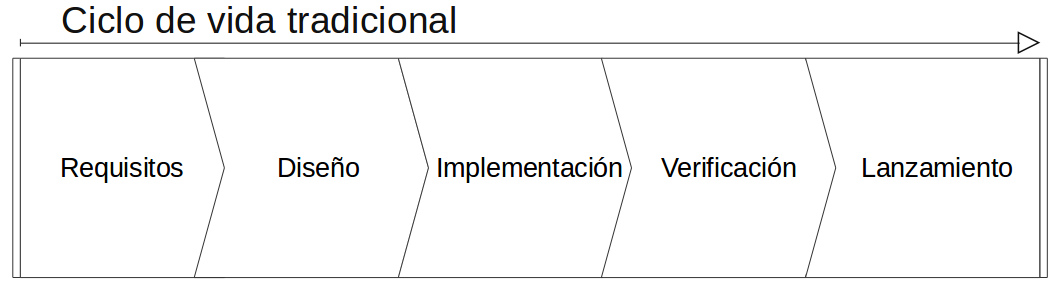
\includegraphics[height=4.0cm, width=12.0cm]{sa_figura_1}
\caption{\gls{CVTS} según Microsoft.}
\label{fig:example}
\end{figure}

A continuación son listadas las actividades propuestas por Microsoft para cada una de las etapas de \gls{SDL}:

\begin{enumerate}
\item Actividades de la etapa de Entrenamiento en Seguridad.
\\
\begin{enumerate}

\item \textit{Entrenamiento sobre seguridad: }practica en la cual es necesario  proveer el conocimiento adecuado e información reciente sobre tópicos de seguridad y privacidad a toda la organización, se debe garantizar que todos los miembros cuentan con los conocimientos necesarios. Los roles que se encuentran directamente relacionados con el desarrollo, es decir, desarrolladores, ingenieros de pruebas, administradores, entre otros, deben de terminar de manera exitosa por lo menos 1 curso o certificación cada año \cite{SDLWhitePaper}. \\

A continuación se listan las temáticas y tópicos que el entrenamiento en seguridad deben cubrir:\\

\begin{enumerate}
\item Diseño seguro
	\begin{enumerate}
		\item Reducción de superficie de ataque
		\item Defensa en lo profundo
		\item Principio de privilegios mínimos
		\item Incumplimiento de seguridad\\
		
	\end{enumerate}
\item Modelo de amenazas
	\begin{enumerate}
		\item Descripción de modelo de amenazas	
		\item Implicaciones del diseño de un modelo de amenazas
		\item Restricciones de codificación en base a un modelo de amenazas\\
		
	\end{enumerate}
\item Codificación segura
	\begin{enumerate}
		\item Desbordamientos de búfer	
		\item Errores aritméticos enteros
		\item Restricciones de codificación en base a un modelo de amenazas
		\item \gls{Cross-Site Scripting}	
		\item Inyección de \gls{SQL}
		\item \gls{Criptografia} débil\\
		
	\end{enumerate}
\item Pruebas de seguridad
	\begin{enumerate}
		\item Diferencias entre pruebas de seguridad y pruebas funcionales		
		\item Evaluación de riesgos	
		\item Métodos de pruebas de seguridad\\
		
	\end{enumerate}
\item Intimidad
	\begin{enumerate}
		\item Tipos de datos de privacidad sensible
		\item Mejores practicas de diseño de privacidad
		\item Evaluación de riesgos
		\item Mejores practicas de desarrollo de privacidad
		\item Mejores practicas de pruebas de privacidad\\
	\end{enumerate}
\end{enumerate}

\begin{figure}
\centering
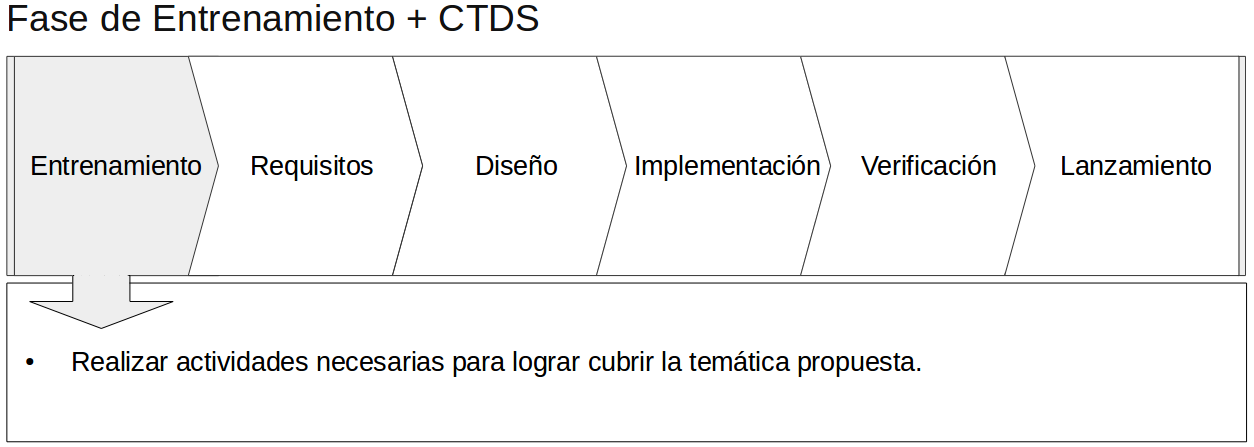
\includegraphics[height=7.0cm, width=12.0cm]{sa_figura_2}
\caption{Fase de entrenamiento añadida al \gls{CVTS}.}
\label{fig:example}
\end{figure}

\end{enumerate}

\item Actividades de la etapa de Requisitos.
\\
\begin{enumerate}
\item \textit{Establecimiento de requisitos de seguridad: }la fase optima para definir requisitos de seguridad es las fase mas temprana del \gls{CVDS} pues se tiene mayor tiempo para identificar hitos y resultados clave, así si mismo se permite una mayor seguridad y privacidad que ayuda a mantener en control las actividades del calendario, se debe realizar una identificación temprana del proyecto y verificar que cumple con alguna de las siguientes características \cite{SDLWhitePaper}:
\\
\begin{enumerate}
	\item ¿El producto que se deberá desarrollar sera sobre algún negocio? 
	\item ¿El producto procesara información confidencial?
	\item ¿El producto contendrá componentes atractivos para menores de edad?
	\item ¿El producto realizara accesos a Internet?
	\item ¿El producto realizara actualizaciones automáticas?\\
	
\end{enumerate}    
Una vez que se ha validado la viabilidad del proyecto sera necesario realizar la determinación de requisitos en base al anterior cuestionario, es decir se deben tomar como premisas claves las respuestas obtenidas con el fin de obtener un correcto listado de los requisitos de seguridad. Se deberá identificar al asesor de seguridad quien fungirá como un primer soporte y quien sera el responsable de definir las políticas globales de seguridad, ademas deberá permanecer al pendiente de cualquier situación que pueda afectar la seguridad del producto. Como siguiente paso sera necesario identificar un ente (persona o equipo) responsable del seguimiento y gestión de la seguridad, su principal responsabilidad sera mantener comunicados e informados acerca del estatus de la seguridad del producto a todos los miembros que conforman el equipo de desarrollo. Después, el asesor de seguridad en conjunto con el equipo de seguridad dueño del producto y cada una de las disciplinas involucradas deberán definir los suficientes requisitos de seguridad para garantizar que el producto funcione adecuadamente en el ambiente operacional requerido, una vez realizado lo anterior se deberá crear un plan adecuado para categorizar y administrar los errores de seguridad relacionados al producto \cite{SDLWhitePaper}. \\

\item \textit{Definir niveles de seguridad y barras de errores: }en esta actividad es necesario establecer los niveles de seguridad y privacidad mínimos que el producto deberá satisfacer, los beneficios de realizar esta actividad son, un mejor entendimiento de los riegos de la seguridad y la privacidad y proveer una base solida de referencia a la hora de depurar errores en la fase de desarrollo. Se deberían establecer niveles mínimos en cada etapa del \gls{CVDS} y dichos niveles deberán ser aceptados por el asesor en seguridad y privacidad \cite{SDLWhitePaper}. \\

\item \textit{Realizar la evaluación de riesgos de seguridad: }todas aquellas organizaciones que se dediquen al desarrollo de Software deberán de realizar una evaluación de riesgos que incluya todas las posibles amenazas y vulnerabilidades, a continuación se listan los tipos de información que dichas evaluaciones deben contener \cite{SDLWhitePaper}: \\
		
\begin{enumerate}
	\item ¿Qué porcentaje del proyecto requiere un modelo de amenazas?
	\item ¿Qué porcentaje del proyecto requiere revisiones del diseño seguro?
	\item ¿Qué porcentaje del proyecto requiere examenes de penetración especializados y si los especialistas son externos?
	\item ¿Exiten requisitos de pruebas o análisis de seguridad adicionales que el asesor considere necesarios para mitigar los riesgos de seguridad?
	\item ¿Cual es el alcance especifico de los requisitos de las \gls{Pruebas Fuzz}?
	\item ¿Cual sera el impacto de la conformidad del producto? (Sera necesario que cada organización emplee su propio \gls{Framework} para medir el impacto).\\
	
\end{enumerate} 
\end{enumerate}
A continuación es presentada de manera gráfica la adición de las actividades de la etapa de requisitos al \gls{CVTS} y a la fase de entrenamiento en seguridad (véase figura 3).
\begin{figure}
\centering
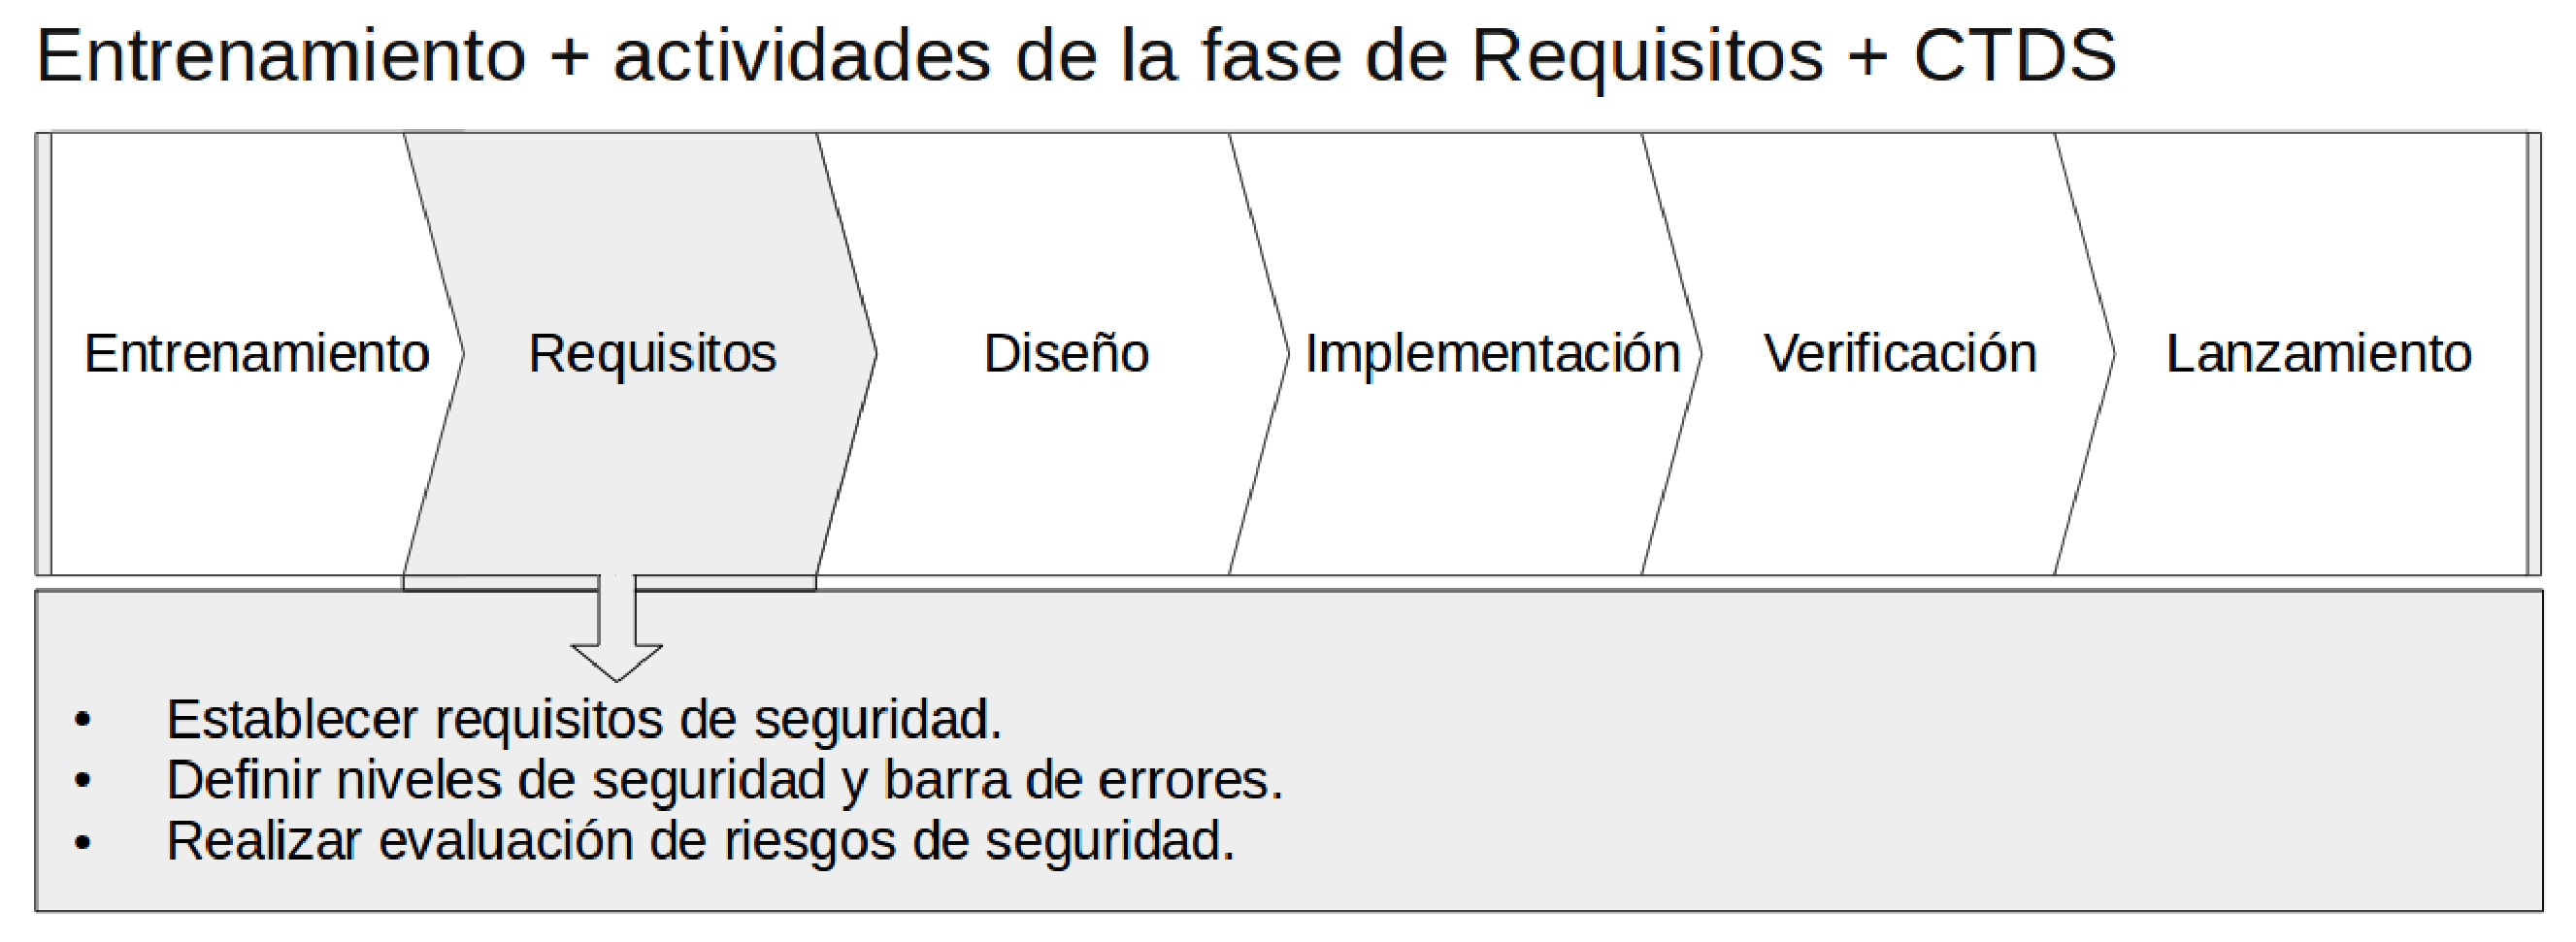
\includegraphics[height=7.0cm, width=12.0cm]{sa_figura_3}
\caption{Actividades de la fase de requisitos añadidas al \gls{CVTS} y a la fase de entrenamiento.}
\label{fig:example}
\end{figure} 


\item Actividades de la etapa de Diseño.
\\
\begin{enumerate}

\item \textit{Establecer los requisitos de diseño seguro: } para establecer los requisitos de diseño seguro es necesario considerar las características de alto riesgo así como establecer técnicas seguras para la codificación, los resultados obtenidos de dichas actividades deben de ser documentados como requisitos de diseño seguro. Es necesario realizar comparativas entre las especificaciones de diseño en contra de las especificaciones funcionales, la especificaciones deben cumplir con la siguiente lista de actividades \cite{SDLWhitePaper}:
\\
\begin{enumerate}
	\item Describir de manera precisa el uso previsto de una característica o función.
	\item Describir cómo implementar la característica o función de una manera segura.
	\item Describir si la característica o función tocarán datos de tarjetas de pago.\\
\end{enumerate}

El control de cambios ofrece un registro archivado para los desarrolladores de aplicaciones pues permite revisar los cambios que los datos de impacto controlado como los datos de tarjetas de pago. La \gls{Criptografia} es una pieza critica en la fase de diseño seguro pues se deben satisfacer de manera obligatoria los mínimos requisitos criptográficos establecidos, entre los cuales se encuentra \cite{SDLWhitePaper}:  
\\
\begin{enumerate}
	\item Usar \gls{AES} para el cifrado y descifrado simétrico. 
	\item Usar 128 bits para mejorar las llaves simétricas.
	\item Usar RSA para el cifrado y descifrado asimétrico y firmas.
	\item Usar llaves RSA de 1024 bits o mejores.
	\item Usar SHA-256 para \gls{Hashing} y códigos de autenticación.\\                                                                        
\end{enumerate}

\item \textit{Análisis de la superficie de ataque: }en esta practica se debe realizar una reducción de la superficie de ataque, en otras palabras, realizar los trabajos para lograr la mínima probabilidad de ser vulnerado entre dichos trabajos se debe encontrar como mínimo los siguientes puntos:\\


\begin{enumerate}
	\item Usar \gls{CAS}.
	\item Administrar las excepciones de \gls{Firewall} cuidadosamente.
	\item Verificar que el producto funciona correctamente para usuarios sin permisos de administrador.\\
\end{enumerate}

\item \textit{Completar el modelo de amenazas: } se debera utilizar el modelo de amenazas con aquellos componentes que fueron identificados como componentes sensibles durante la fase de evaluación de riesgos de seguridad. Poner el practica el modelo de amenazas permite al equipo de desarrollo mantener control sobre las implicaciones de seguridad dentro de un ambiente operacional. Los trabajos deben ser realizados con el equipo completo, dichos trabajos pueden ser listados de la siguiente manera \cite{SDLWhitePaper}:
\\
\begin{enumerate}
	\item Completar el modelo de amenazas para los componentes sensibles  o componentes que tienen riegos y los cuales fueron identificados en la fase de evaluación de riesgos de seguridad. \\
	
	Los modelos de amenazas deben considerar las siguientes areas: \\
	
	\begin{enumerate}
		\item Todos los proyectos, todo el código que se exponen en la superficie de ataque así como el código que sea escrito por entidades externas al equipo de desarrollo. 
		\item Proyectos nuevos, todas las características y funcionalidades.
		\item Versiones actualizadas, todas las características y funcionalidades agregadas.\\
	\end{enumerate}
	\item Verificar que el modelo de amenazas es el adecuado para satisfacer los requisitos mínimos de calidad.
	\item Verificar que el modelo de amenazas contiene la información necesaria, diagramas de flujo, activos, vulnerabilidades y formas de mitigacion.
	\item Realizar el modelo de amenazas utilizando \gls{STRIDE}, técnica de descomposición de componentes.
	\item Utilizar las herramientas propuestas por Microsoft en su sitio oficial.
	\item Asegurarse que los resultados de cada trabajo sea aprobado por un experto en seguridad. \\
\end{enumerate}

La documentación generada en esta practica debe encontrarse almacenada y disponible para futuras revisiones en la fase de verificación. \\

\end{enumerate}

A continuación es presentada de manera gráfica la adición de las actividades de la etapa de diseño al \gls{CVTS} y a la fase de entrenamiento en seguridad (véase figura 4).\\

\begin{figure}
\centering
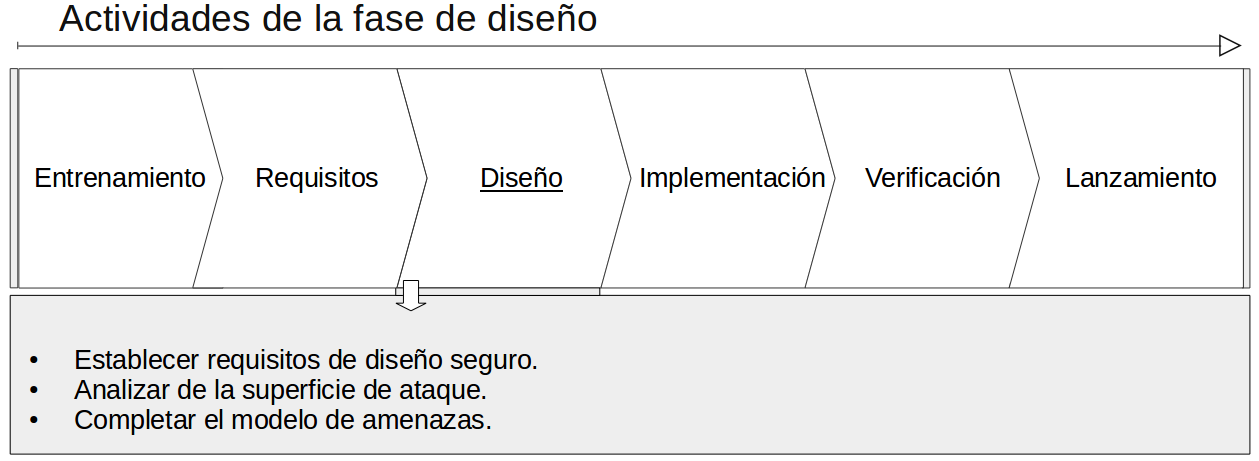
\includegraphics[height=6.0cm, width=12.0cm]{sa_figura_4}
\caption{Actividades de la fase de diseño añadidas al \gls{CVTS} y a la fase de entrenamiento.}
\label{fig:example}
\end{figure}

\item Actividades de la etapa de Implementación.
\\
\begin{enumerate}
	\item \textit{Utilizar herramientas aprobadas: }se deberá utilizar herramientas aprobadas por el asesor en seguridad, se debe mantener una lista publicada de las herramientas para que todos los miembros del equipo puedan consultarla en cualquier momento, se deberán utilizar las versiones mas resientes para aprovechar las nuevas funcionalidades y protecciones \cite{SDLWhitePaper}. \\
	
	\item \textit{Depreciar funciones no seguras: }se deberá determinar cuales serán las funciones inseguras vetadas, el equipo deberá utilizar cabeceras para detectar cualquier función insegura vetada y compiladores nuevos así como herramientas de análisis de código automáticas que permitan identificar el uso de funciones inseguras \cite{SDLWhitePaper}. \\
	
	\item \textit{Realizar análisis estáticos: }se deberá realizar un análisis estático a código fuente, el asesor de seguridad deberá evaluar el uso de herramientas automáticas para la revisión del código o revisiones humana que promuevan la remoción de vulnerabilidades \cite{SDLWhitePaper}.   
\\
\end{enumerate}

A continuación es presentada de manera gráfica la adición de las actividades de la etapa de implementacion al \gls{CVTS} y a la fase de entrenamiento en seguridad (véase figura 5).
\begin{figure}
\centering
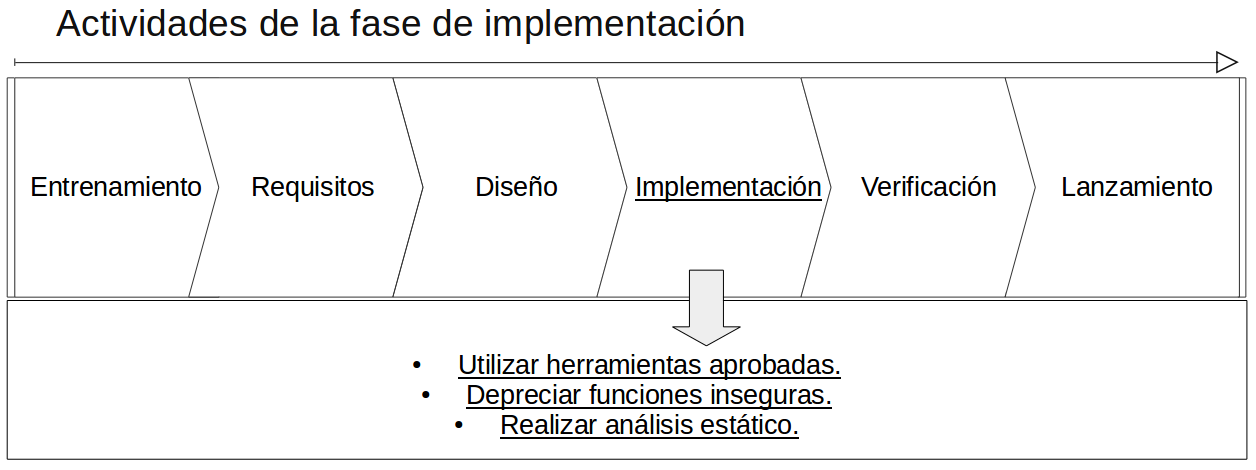
\includegraphics[height=6.0cm, width=12.0cm]{sa_figura_5}
\caption{Actividades de la fase de implementacion añadidas al \gls{CVTS} y a la fase de entrenamiento.}
\label{fig:example}
\end{figure} 
\\
\item Actividades de la etapa de Verificación.
\\
\begin{enumerate}
	\item \textit{Realizar análisis de código dinámico: }se deberán realizar verificaciones en tiempo de ejecución para verificar que el funcionamiento es el diseñado, se deberá especificar que tipo de herramientas  podrán utilizarse para el monitoreo del comportamiento del producto \cite{SDLWhitePaper}. \\ 
	
	\item \textit{Realizar \gls{Pruebas Fuzz}: }estas son realizadas por medio de la inserción de información mal formada o al azar con el fin de producir errores en el producto \cite{SDLWhitePaper}. \\
	
	\item \textit{Realizar una revisión de la superficie de ataque: }para evitar vulnerabilidades producidas por la desviación funcional del producto y el diseño del mismo se deberá realizar revisiones al modelo de amenazas y a la superficie de ataque \cite{SDLWhitePaper}. \\
\end{enumerate}
A continuación es presentada de manera gráfica la adición de las actividades de la etapa de implementación al \gls{CVTS} y a la fase de entrenamiento en seguridad (véase figura 6). \\
\begin{figure}
\centering
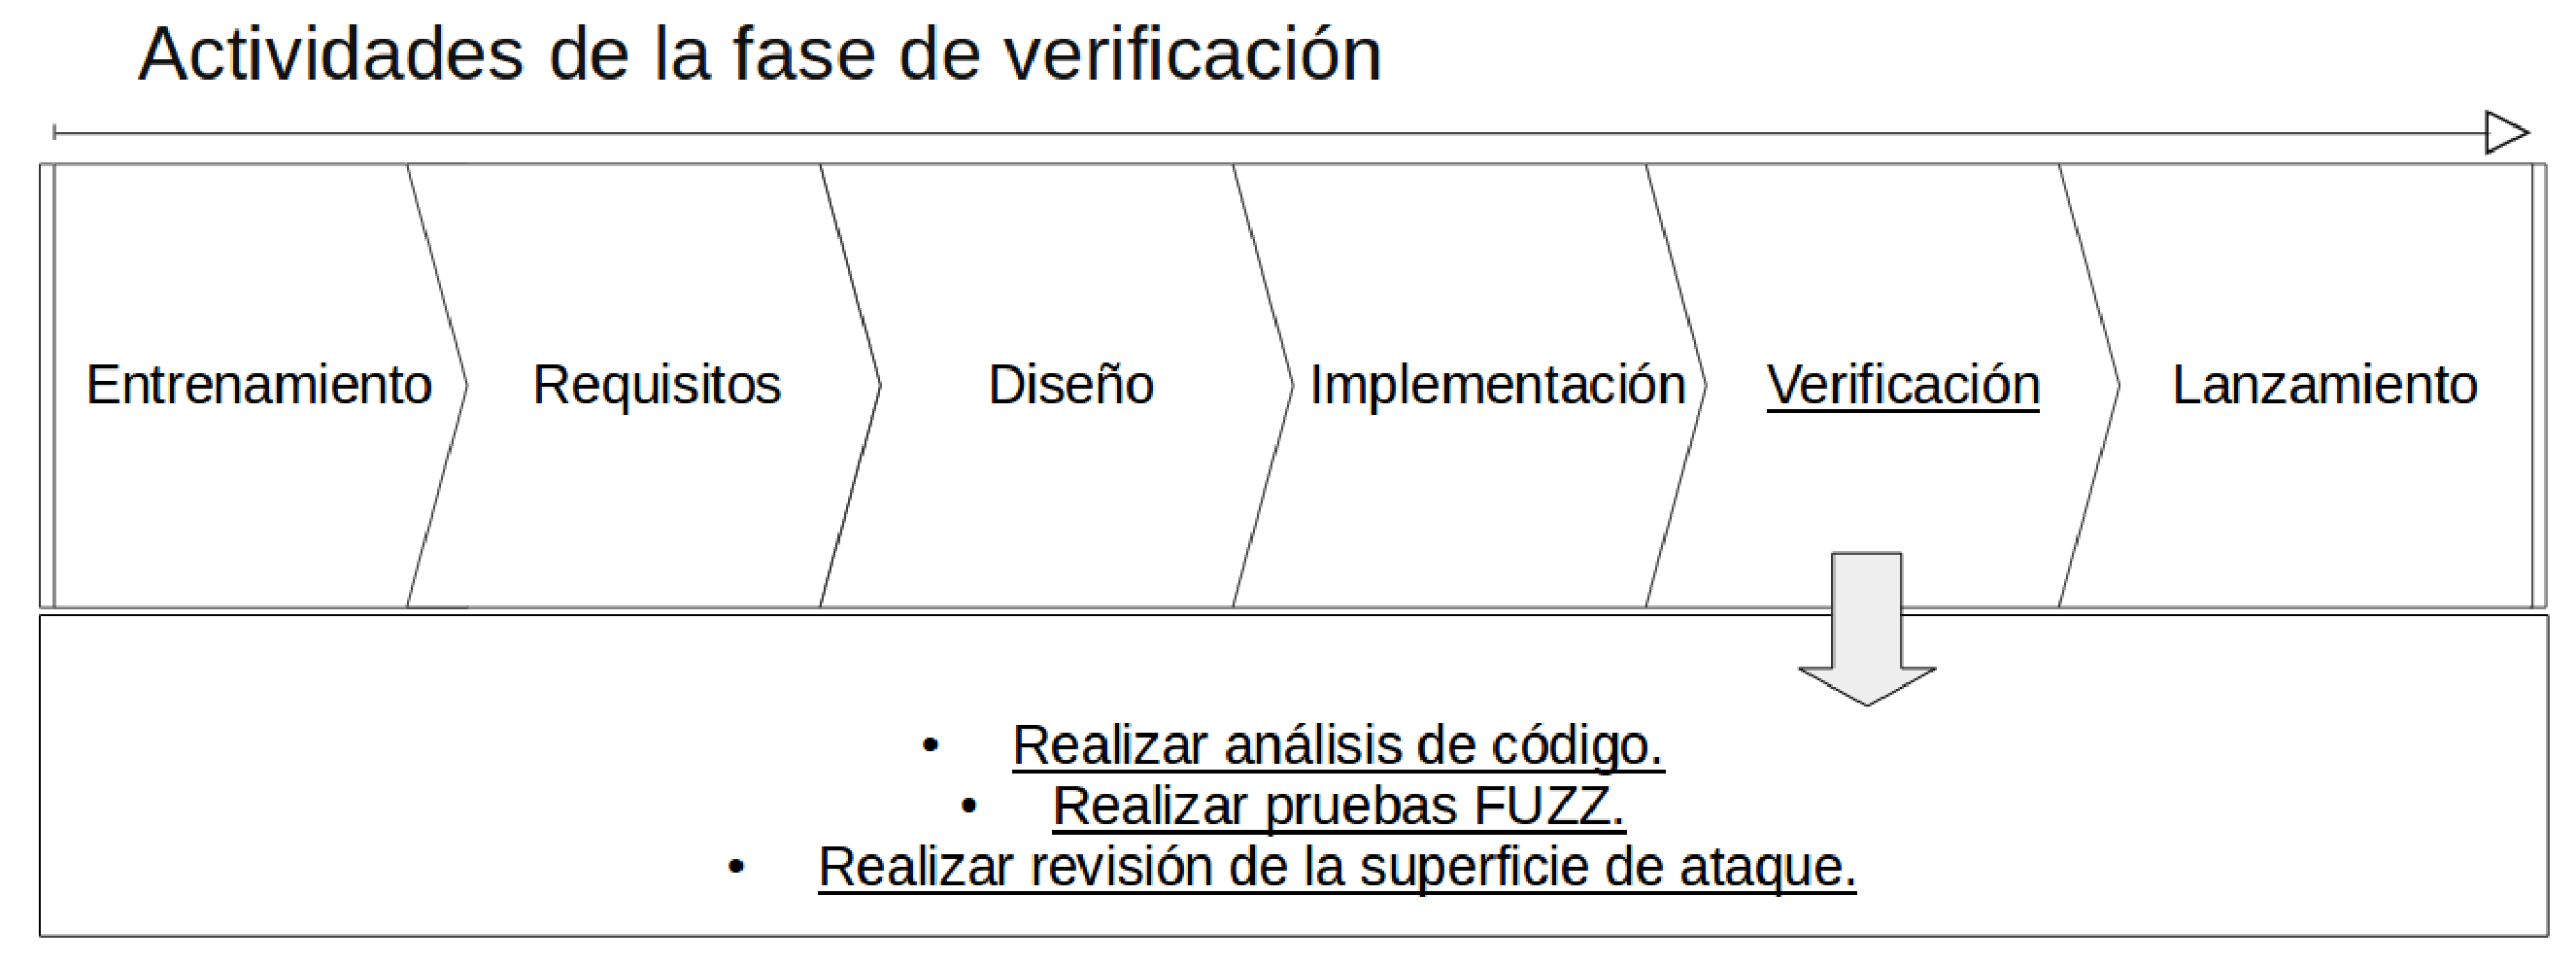
\includegraphics[height=6.0cm, width=12.0cm]{sa_figura_6}
\caption{Actividades de la fase de verificación añadidas al \gls{CVTS} y a la fase de entrenamiento.}
\label{fig:example}
\end{figure} 

\item Actividades de la etapa de Lanzamiento.
\\
\begin{enumerate}
	\item \textit{Crear un plan de respuesta a incidentes: }debido a la incertidumbre sobre futuras vulnerabilidades emergentes el plan de respuesta deberá incluir los siguientes puntos \cite{SDLWhitePaper}: \\
	\begin{enumerate}
		\item Una lista de la información de contacto de quien servirá como primer contacto ante una emergencia.	
		\item Información de contacto de autoridades para la toma de decisiones 24 horas al día 7 días a la semana.		
		\item Planes de servicio de seguridad (procedimientos de escalamiento) de código heredado de otros grupos dentro de la organización.		
		\item Planes de servicio de seguridad (procedimientos de escalamiento) de código de terceros con licencia, incluyendo los nombres de archivos, versiones, código fuente, información de contacto con otros proveedores, y autorización contractual para realizar cambios (en su caso).\\
		\end{enumerate}
	
	\item \textit{Realizar un revisión final de la seguridad: }no es un examen de penetración, no es una forma de mitigar problemas de seguridad olvidados, la revisión final incluye examinar el modelo de amenazas,  
las solicitudes de excepción, las salidas de la herramientas y el desempeño contra los niveles de calidad previamente determinadas \cite{SDLWhitePaper}. \\

Existen dos tipos de revisiones finales de la seguridad y pueden ser listados de la siguiente manera:\\
	\begin{enumerate}
		\item Pasada: todos los problemas de seguridad identificados han sido arreglados.
		\item Pasada con excepciones: todos los problemas de seguridad identificados han sido arreglados y las escepciones resueltas, aquellas que no puedan abordarse deran ser arregladas en la siguiente version del producto, si existe alguna escepcion esta tiene que ser revisada por el asesor de seguridad, el asesor tiene que llegar a algún compromiso con el dueño del producto y si no lo logra el producto no deberá ser liberado. \\
\end{enumerate}
	
\item \textit{Archivar la información: }para mejorar la velocidad y la calidad de respuesta durante un incidente se deberá incluir los siguientes puntos: \\
	\begin{enumerate}
		\item Especificación de características.		
		\item Código fuente, binarios y símbolos privados.		
		\item modelos de amenazas.		
		\item Casos de prueba.		
		\item Documentación relacionada.		
		\item Planes de respuesta.	
		\item Licencias y términos de servicios para cualquier producto de terceros.\\
	\end{enumerate}

\end{enumerate}

A continuación es presentada de manera gráfica la adición de las actividades de la etapa de liberación al \gls{CVTS} y a la fase de entrenamiento en seguridad (véase figura 7).\\

\begin{figure}
\centering
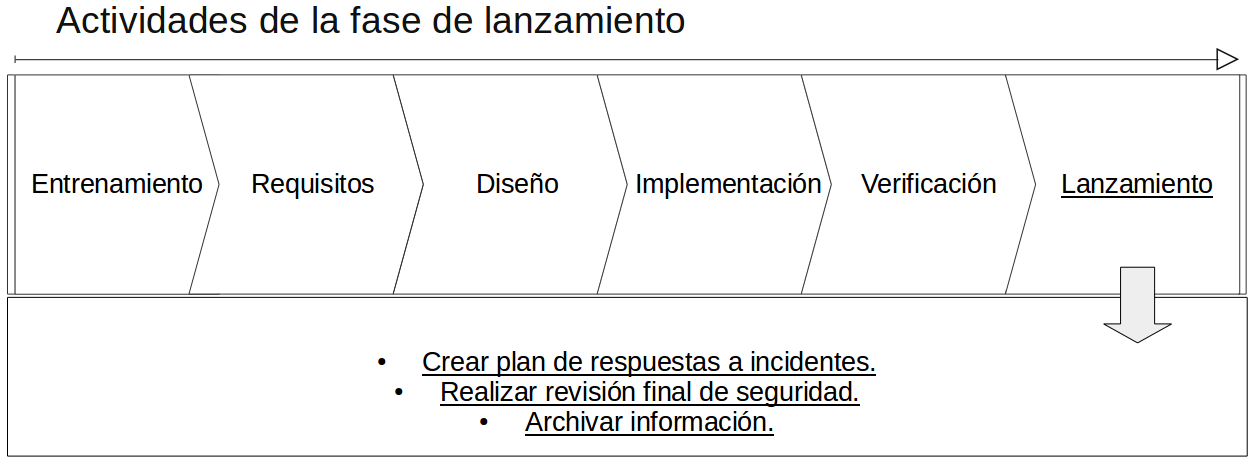
\includegraphics[height=6.0cm, width=12.0cm]{sa_figura_7}
\caption{Actividades de la fase de lanzamiento añadidas al \gls{CVTS} y a la fase de entrenamiento.}
\label{fig:example}
\end{figure} 


\item Actividades de la etapa de Respuesta.
\\
\begin{enumerate}
	\item \textit{Ejecutar plan de respuesta a incidentes: } se deberán poner en practica las actividades planeadas con anterioridad como respuesta a cualquier ataque, sospecha o amenaza (véase figura 8) \cite{SDLImplementacionSimplificada}.
\end{enumerate}

\begin{figure}
\centering
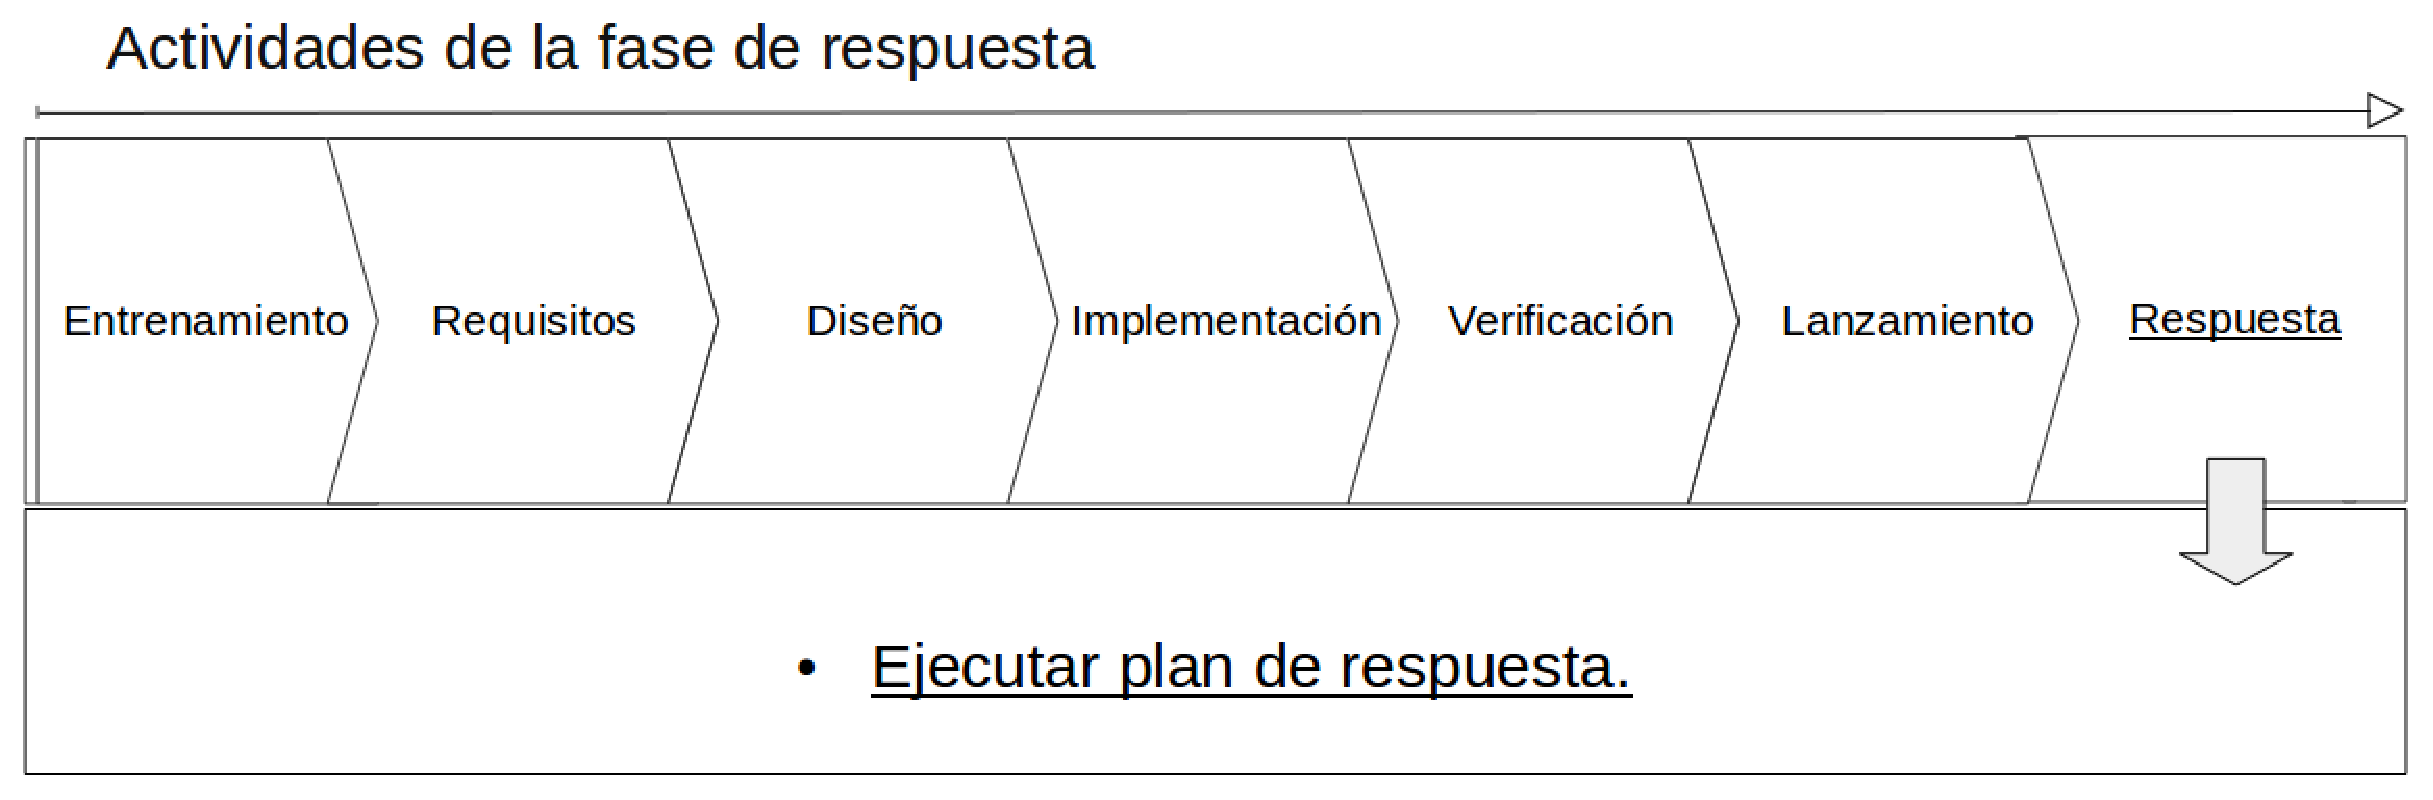
\includegraphics[height=6.0cm, width=12.0cm]{sa_figura_8}
\caption{Actividades de la fase de respuesta añadidas al \gls{CVTS} y a la fase de entrenamiento.}
\label{fig:example}
\end{figure} 
\end{enumerate}

\gls{SDL} fue creado como un proceso del cual cualquiera puede disponer, su principal meta es mejorar de manera drástica la seguridad y la privacidad de la información contenida en los productos desarrollados bajo su dirección, \gls{SDL} posee acciones obligatorias sin embargo es posible integrar en su proceso actividades o directivas privadas con el fin de construir una metodología única para cada organización. Las aportaciones que la nueva metodología deberá combinar son, los procesos, la formación y las herramientas especializadas, que en conjunto deberán producir mayor previsibilidad y capacidad técnica así como un producto mas seguro lo cual se vera reflejado en un menor riesgo para la organización y el usuario final del producto.

\subsubsection{¿Por qué adoptar \gls{SDL}?}
Internet, o como algunos la llamarían \textit{The World Wide Web} se ha convertido en el mayor medio de comunicación, pues ha logrado congregar a centenas de miles de usuarios que conectados entre si comparten e intercambian información al mismo tiempo \cite{webAplicationSecurity}. En la actualidad existe una demanda continua de nuevos medios seguros de comunicación a través de la red, debido a ello los productores de Software requieren de innovadoras técnicas que garanticen la producción de Software seguro y ademas de ello contengan características adecuadas para una rápida y correcta adopción lo cual se deberá ver reflejado en el aspecto económico de la empresa. \\

\gls{SDL} posee características únicas que pueden ser aprovechadas para lograr una correcta y rápida inserción en el trabajo, algunas de importancia son listadas a continuación \cite{webAplicationSecurity}: 
\begin{enumerate}
	\item \gls{SDL} es definido como sus creadores como un proceso que puede ser adaptado a cualquier técnica utilizada para desarrollar Software de calidad.
	\item  \gls{SDL} esta diseñado para cualquier tamaño de empresa.
	\item \gls{SDL} presenta una documentación \gls{Online} en varios idiomas.
	\item  Cada tópico de importancia es abordado a detalle.
	\item  \gls{SDL} promueve el cumplimiento de los estándares ISO/IEC 27034-1 y ISO/IEC 27034-1:2011.
\end{enumerate}

\subsubsection{¿Cómo adoptar \gls{SDL}?}
Para lograr una correcta adopción de \gls{SDL} es necesario seguir de manera puntual 7 pasos o etapas que han sido establecidos por Microsoft pues se ha logrado recopilar información valiosa a lo largo de varios años de practica dentro de los sectores financieros de alto riesgo. A continuación son presentadas dichas etapas \cite{SDLWhitePaper}: 

\begin{enumerate}
\item Educacion 
\item Personalización 
\item Conocimiento de herramientas e infraestructura 
\item Entrenamiento 
\item Puesta en marcha 
\item Medición 
\item Revisión 
\end{enumerate}

La fase de educación es sumamente importante, en su mayoría los expertos reconocen que la correcta comprensión de la información acerca de \gls{SDL} por parte de los equipos de desarrollo es la llave para la correcta adopción pues es necesario comprender de manera detallada como es que cada uno de los puntos de inserción embonan con las actividades y esfuerzos realizados cotidianamente dentro de la organización, es decir, en esta etapa es necesario asegurarse que dentro de la organización existe un conocimiento pleno sobre \gls{SDL}. \\

La fase de personalización es utilizada para lograr la correcta estructuración y conexión entre el ciclo de vida de desarrollo de Software cotidiano y \gls{SDL}, es decir, se debe comprender de manera detalla cuales son las actividades o fases que serán incluidas en el \gls{CVDS} utilizado en la organización pues \gls{SDL} esta diseñado para ajustarse y moldearse a conveniencia de los interesados \cite{SDLWhitePaper}. \\

La fase de conocimiento de herramientas e infraestructura hace énfasis en establecer normativas de uso y disposición de herramientas enfocadas en mejorar el proceso de adopción de \gls{SDL}, el equipo deberá conocer a fondo las herramientas que serán utilizadas ademas de establecer un correcto entorno de desarrollo. Microsoft ofrece una amplia gama de herramientas libre de cargo que están enfocadas en mejorar la correcta inserción y uso de \gls{SDL} y las cuales pueden ser encontradas \gls{Online} en el siguiente \gls{URL}: \url{http://www.microsoft.com/en-us/sdl/adopt/tools.aspx}. \\

La fase de entrenamiento considera necesario realizar una introducción informativa general a todos los miembros de la organización con el fin de promover el conocimiento de las actividades que serán puestas en practica, se deberá considerar que sera necesario realizar sesiones de entrenamiento para cada tipo de rol o para aquellos roles que tengan responsabilidades de alta jerarquía. Los expertos consideran que los entrenamientos específicos deberán ser llevados acabo una vez que los miembros de la organización ya estan utilizando \gls{SDL} \cite{SDLWhitePaper}. \\

La fase de puesta en marcha debe ser monitoreada constantemente pues es aquí cuando la mayoría de las problemáticas surgen y es cuando sera necesario evaluar las nuevas acciones realizadas con el fin de realizar modificaciones o adaptaciones que resulten en mejoras continuas al proceso \cite{SDLWhitePaper}. \\

La fase de medición esta dedicada en analizar de manera detallada los resultados obtenidos de dos principales practicas y las cuales son mencionadas a continuación:

\begin{enumerate}
\item Revisión final de seguridad 
\item Postmortem 
\end{enumerate}

El cometido principal de estas practicas es eliminar cualquier tipo de defecto en la seguridad de los productos antes de llegar al cliente, todo esto por medio de comparativas con modelos de riesgos, administración de historiales de defectos entre otros. De esta manera es posible tener una base contable sobre los resultados obtenidos a través del tiempo promoviendo así la mejora continua del proceso. \\

En la fase de revisión se deberán llevar a cabo análisis formales de los datos recavados en la fase anterior con el principal objetivo de promover mejoras del proceso por medio de modificaciones a las actividades, a dichas revisiones deberán asistir todos los involucrados \cite{SDLWhitePaper}. 

\subsubsection{¿Cómo evaluar el impacto de \gls{SDL}?}

Para lograr la inserción de conceptos o modificaciones a los procesos y lograr productos mas seguros es necesario realizar la acciones correspondientes, las variables que juegan un papel importante para lograr escalar dentro de los niveles de madurez de cualquier modelo son el tamaño de la organización, los recursos como el tiempo, talento y presupuestos además claro del respaldo de los directivos,  para obtener un correcto control de los impacto intangibles es necesario lograr una comprensión detallada de los elementos que constituyen los procedimientos de desarrollo de seguridad y establecer normas de implementación según el nivel de madurez que el equipo de desarrollo posea, \gls{SDL} posee su propio modelo de optimización el cual ayuda en todas las cuestiones anteriormente mencionadas. El modelo esta constituido por 5 áreas de capacidades las cuales corresponden con el \gls{CVDS} y las cuales pueden ser  mencionadas de la siguiente manera \cite{SDLSecurityDevelopmentLifecicle}: 

\begin{enumerate}
	\item Formación, políticas y capacidades organizativas 
	\item Requisitos y diseño 
	\item Implementación 
	\item Comprobación 
	\item Lanzamiento y respuesta 
\end{enumerate}

A continuación son listados los niveles de madurez utilizados por el modelo \gls{SDL}:

\begin{enumerate}
\item Básico 
\item Dinámico 
\item Estandarizado 
\item Avanzado 
\end{enumerate}

El modelo comienza en nivel básico en el cual la organización posee pocos procesos, cursos de formación y herramientas, este nivel tiene como cometido poder llevar a la organización al nivel dinámico en el cual la misma poseerá procesos eficaces, personal altamente cualificado, herramientas especializas y un alto grado de responsabilidad por parte de los involucrados internos y externos, en este orden se pretende llegar al nivel superior conocido como nivel avanzado (véase figura 9). \\

\begin{figure}
\centering
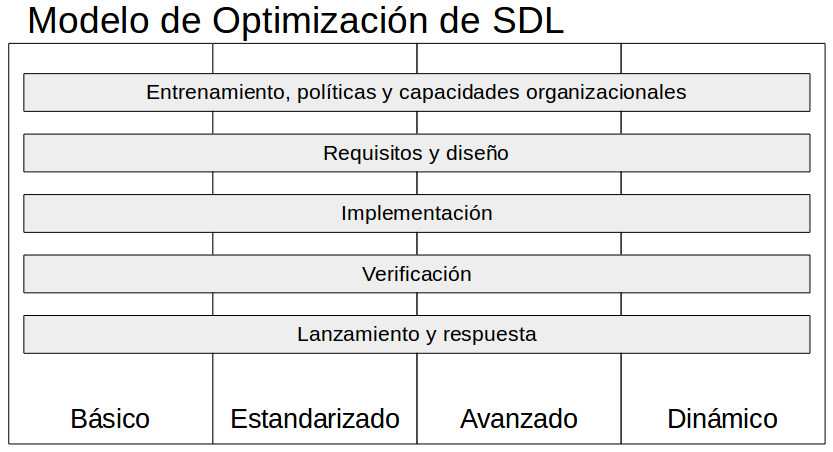
\includegraphics[height=7.2cm, width=12.0cm]{sa_figura_9}
\caption{Modelo de optimización utilizado por \gls{SDL}.}
\label{fig:example}
\end{figure}


\subsubsection{¿Quiénes deben poner en practica \gls{SDL}?}
Microsoft propone una lista de características que los proyectos deben tener para ser candidatos ideoneos seguir un proceso \gls{SDL}.

\begin{enumerate}
	\item Aplicaciones que procesan datos de identificación personal o cualquier otro  tipo de información confidencial o privilegiada. 
	\item Aplicaciones que se comunican o realizan envíos de información frecuentemente a través de Internet u otros redes. 
	\item Aplicaciones implementadas en entornos empresariales.
\end{enumerate}

\subsubsection{¿Cuáles son las cualidades de \gls{SDL}?}
Las cualidades que \gls{SDL} posee según el estudio realizado por Ikram El rhaffari y Ounsa Roudies y el cual esta enfocado en el análisis de elementos pertenecientes a la Ingeniería de \gls{Software}, a la Seguridad Informática y a las \gls{IT} y son listadas a continuación \cite{BenchmarkingSDLCLAPS}. 

\begin{enumerate}
	\item Cualidades relacionadas a la Ingeniería de \gls{Software}.
		\begin{enumerate}
			\item El producto final tendrá varios enfoques de calidad.
			\item El mapeo al \gls{CVTS} es facil.
			\item Se alinea fácilmente con otros métodos de Ingeniería de \gls{Software}.
			\item La información para la implementación y los recursos necesarios se encuentran \gls{Online}.
			\item Posee su propia guía para el desarrollo de actividades.\\
			
		\end{enumerate}
	\item Cualidades relacionadas a la Seguridad Informática.
		\begin{enumerate}
			\item Posee un enfoque basado en promover la seguridad para alcanzar la calidad.
			\item Implica y compromete a un equipo de seguridad y promueve la interacción entre los actores.
			\item Posee un bajo indice de cumplimiento y privacidad.\\
			
		\end{enumerate}
	\item Cualidades relacionadas con \gls{IT}.
		\begin{enumerate}
			\item Se enfoca en promover la calidad.
			\item Su documentación posee un alto indice de completitud y se encuentra disponible de manera \gls{Online}.
			\item Provee una completa cobertura organizacional.
			\item Es evolutivo.
			\item Se adapta fácilmente a diferentes tipos de estructuras organizacionales.
			\item Posee su propio modelo de madurez.
			\item Provee soporte para el aseguramiento de la calidad de los servicios.\\
		\end{enumerate}
\end{enumerate}

El proceso promueve la mejora continua en las organizaciones ayudándolas alcanzar la certificación ISO/IEC 27034-1 la cual garantiza que la organización mantiene procesos que involucran la aplicación de controles, medidas y mediciones con el fin de gestionar el riesgo de uso de los productos desarrollados \cite{SDLWhitePaper}. 

\subsubsection{¿Cuáles son las deficiencias que presenta \gls{SDL}?}
Las deficiencias que \gls{SDL} posee según el estudio realizado por Ikram El rhaffari y Ounsa Roudies y el cual esta enfocado en el análisis de elementos pertenecientes a la Ingeniería de \gls{Software}, a la Seguridad Informática y a las \gls{IT} y son listadas a continuación \cite{BenchmarkingSDLCLAPS}. 

\begin{enumerate}
	\item Deficiencias relacionadas a la Ingeniería de \gls{Software}.
		\begin{enumerate}
			\item No es \gls{Flexible} y es riguroso.\\
			
		\end{enumerate}
	\item Deficiencias relacionadas a la Seguridad Informática.
		\begin{enumerate}
			\item No posee métricas de seguridad.\\
			
		\end{enumerate}
	\item Deficiencias relacionadas con \gls{IT}, no presenta deficiencias de acuerdo al estudio de Ikram El rhaffari y Ounsa Roudies \cite{BenchmarkingSDLCLAPS}.
		
\end{enumerate}

\subsection{Proceso de Seguridad en Aplicación Completo y Ligero}
Comprehensive, Lightweight Application Security Process (CLASP, Proceso de Seguridad en Aplicación Completo y Ligero), es un proyecto creado como parte de \gls{OWASP} bajo la supervision de Pravir Chandra en colaboración de Jeremy Feragamo, Dan Graham, John Viega, Jeff Williams y Alex Newman. \gls{CLASP} es un recurso que se encuentra bajo licencia \gls{Open Source}, sus responsables hacen una invitación abierta a todos los profesionales relacionados a la seguridad informática a realizar aportaciones y revisiones del material existente por medio de la inscripción a una membresia de bajo coste \cite{CLASPIntroduction}.

\subsubsection{¿Qué es \gls{CLASP}?}
\gls{CLASP} es definido como un conjunto de piezas de proceso que pueden ser adoptadas para trabajar en conjunto con ciclos de vida de desarrollo de \gls{Software} definidos. La meta principal que persigue \gls{CLASP} es proveer de una estructura fiable para la depuración de problemáticas relacionadas a la seguridad en fases tempranas del \gls{CVDS} \cite{CLASPIntroduction}. 
\\\\
\gls{CLASP} esta formado por una gran cantidad de recursos extraídos de Ciclos de Vida de Desarrollo de \gls{Software} los cuales metódicamente fueron descompuestos para crear un conjunto de requisitos de seguridad que son la base de las mejores practicas de \gls{CLASP} y las cuales permiten a las organizaciones a soluvionar vulnerabilidades de manera sistemática. Las actividades para la mejora de la seguridad de \gls{CLASP} fueron diseñadas para ser integradas facilmente con otros procesos de desarrollo existentes, cada una de estas actividades deberá ser asignada a uno o mas roles, \gls{CLASP} provee una guía para los participantes del proceso. \gls{CLASP} provee un \gls{LV} propio el cual esta diseñado para ayudar a los equipos de desarrollo a abordar y remediar errores específicos de diseño o codificación que puedan ser explotados \cite{CLASPConcepts}.  
\\\\
La estructura de componentes \gls{CLASP} y sus dependencias se organizan de la siguiente manera:

\begin{enumerate}
	\item Vistas \gls{CLASP}.\\\\
	Existen 5 tipos de vistas que son consideradas perspectivas de alto nivel, cada vista es dividida en 			componentes de proceso por medio de una organización del tipo (Vista - Actividad - Componente de 			    Proceso).\\
	
	Las vistas \gls{CLASP} son listadas a continuación.\\
	
		\begin{enumerate}
			\item \gls{VC}
			\item \gls{VBR}
			\item \gls{VBEA}
			\item \gls{VBIA}
			\item \gls{VV}\\
			
		\end{enumerate}
Para lograr obtener una idea clara sobre las interacciones entre componentes es necesario visualizar el diagrama propuesto por \gls{OWASP} (Véase figura 10).\\
	
\begin{figure}
\centering
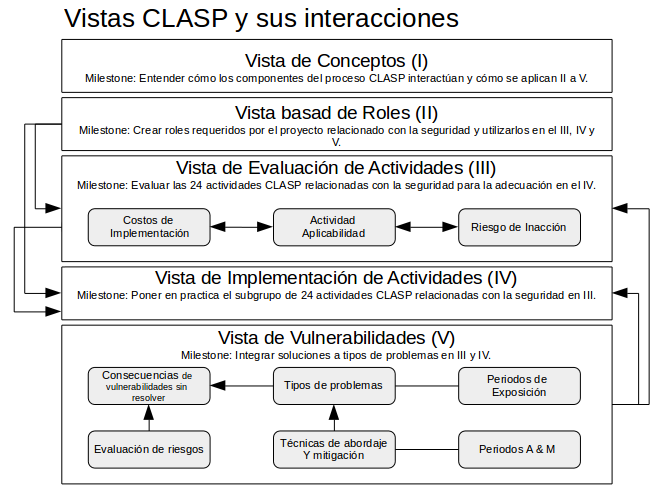
\includegraphics[height=13.0cm, width=12.0cm]{sa_figura_10}
\caption{Vistas \gls{CLASP} y sus interacciones.}
\label{fig:example}
\end{figure}
	
	\item Recursos \gls{CLASP}.\\\\ 
	Los recursos propuestos por \gls{CLASP} proveen artefactos útiles cuando en el proyecto que se debe 			desarrollar se utilizan herramientas que automatizan las piezas del proceso \gls{CLASP} \cite{CLASPConcepts}.\\
	
	  A continuación se muestra de manera gráfica el nombre y la localización de los recursos \gls{CLASP} asi como las vistas que cada uno de ellos soporta (véase figura 11).\\
	  
\begin{figure}
\centering
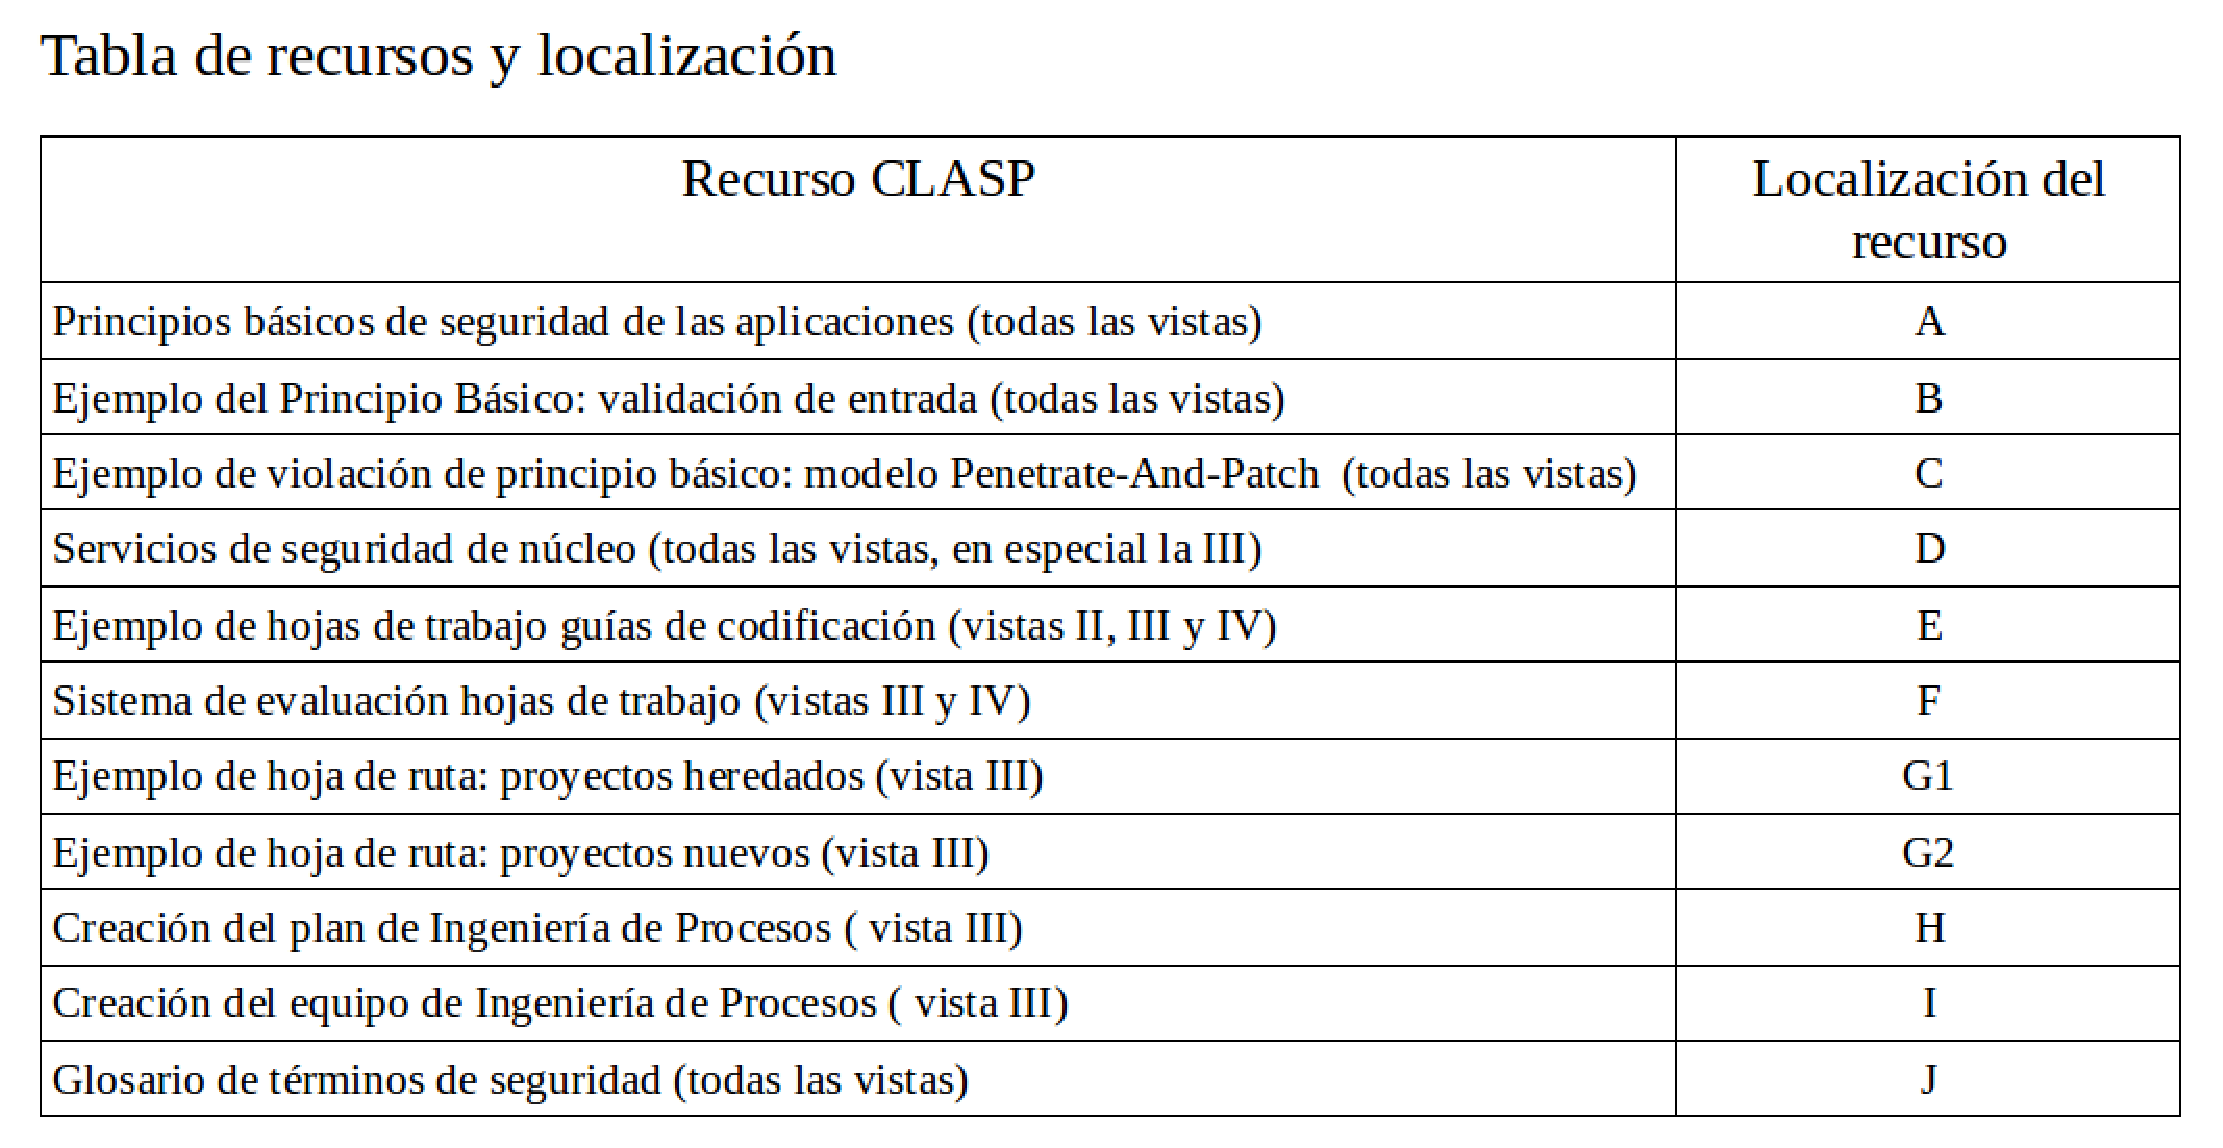
\includegraphics[height=7.0cm, width=12.0cm]{sa_figura_11}
\caption{Recursos \gls{CLASP} y su localización}
\label{fig:example}
\end{figure}
	 
	\item \gls{CUV}.\\\\
	Los \gls{CUV} describen las condiciones bajo las cuales los servicios de seguridad pueden ser vulnerados, 	ademas proporcionan a los usuarios ejemplos de las relaciones causa y efecto entre seguridad / diseño y 		código fuente, así como las vulnerabilidades resultantes en los servicios básicos de seguridad es decir., 	autenticación, autorización, confidencialidad, disponibilidad, responsabilidad, y no repudio \cite{CLASPConcepts}.\\
	
	Los \gls{CUV} están basados en la siguiente lista de arquitecturas de componentes.\\
	
\begin{enumerate}
	\item Monolithic \gls{UNIX}
	\item Monolithic Mainframe
	\item Arquitectura distribuida 
	\\
\end{enumerate}
Los \gls{CUV} deben ser utilizados como un puente entre la \gls{VC} y el \gls{LV} \cite{CLASPConcepts}.
\\	
	\item Mejores practicas.\\\\
	\gls{CLASP} posee 7 practicas enfocadas en la mejora de la aplicación de la seguridad, estas son:\\

	\begin{enumerate}
		\item Realizar programas de sencibilización 
		\item Realizar evaluaciones
		\item Capturar requisitos de seguridad
		\item Construir procedimientos de remediación a vulnerabilidades
		\item Definir y monitorear métricas
		\item Publicar reglas de seguridad operativa\\
		
	\end{enumerate}
\end{enumerate} 
Una vista de alto nivel al orden de ejecución de actividades relacionadas a las políticas de seguridad puede promover el aumento de la conciencia sobre la aplicación de actividades para la mejora de la seguridad. El orden ascendente de ejecución de actividades en la organización puede ser listado de la siguiente manera \cite{CLASPConcepts}:
\\
\begin{enumerate}
	\item Mejores practicas para la aplicación de la seguridad
	\item Políticas para la aplicación de la seguridad
	\item Políticas de seguridad de \gls{IT}
	\item Operación de políticas de seguridad
	\item Políticas de seguridad corporativas\\
	
\end{enumerate}
\gls{CLASP} define \gls{VS} como una debilidad en un entorno de \gls{Software} y define Consecuencia como un fallo en los siguientes servicios básicos de seguridad: 
\\
\begin{enumerate}
	\item Autorización (control de acceso a los recursos)
	\item Confidencialidad (en los datos y otros recursos)
	\item Autenticación (establecimiento de identidad e integridad)
	\item Disponibilidad (denegación de servicios)
	\item Responsabilidad
	\item No repudio\\
	
\end{enumerate}
 \gls{CLASP} posee su propia \gls{Taxonomia} la cual se describe como una clasificación de alto nivel que se divide en clases para una mejorar la evaluación y resolución de las Vulnerabilidades de Seguridad del código fuente \cite{CLASPConcepts}.
\\\\
Las clases en las que se divide son las siguientes.
\\
\begin{enumerate}
	\item Tipos de problemas
	\item Categorías
	\item Periodos de exposición
	\item Consecuencias
	\item Plataformas
	\item Recursos
	\item Evaluaciones de riesgos
	\item Forma de abordaje y periodos de mitigación
\end{enumerate}

\subsubsection{¿Porqué adoptar \gls{CLASP}?}
Entre los principales atractivos que \gls{CLASP} se encuentran sus principios básicos los cuales están enfocados en las determinaciones de \gls{FOSS} y los cuales pueden ser listados de la siguiente manera \cite{CLASPConcepts}:

\begin{enumerate}
	\item Es libre y abierto. 
	\item Es gobernado por consenso áspero y código funcional.
	\item Obliga a cumplir con un código de ética.
	\item No tiene fines de lucro.
	\item No es impulsado por intereses comerciales.
	\item Posee un enfoque basado en el riesgo.
\end{enumerate}

\subsubsection{¿Cómo adoptar \gls{CLASP}?}
\gls{CLASP} ha sido concebido como un conjunto de piezas de proceso que pueden ser adoptadas por cualquier compañía e insertadas en cualquier \gls{CVDS} definido, \gls{CLASP} en su \gls{VBEA} menciona que debido a la gran cantidad de piezas existentes ciertas organizaciones podrían creer que los esfuerzos necesarios para lograr una correcta inserción de las mismas podría acarrear inversiones peligrosas, sin embargo tal y como se menciona en el sitio oficial de \gls{OWASP}, "No es necesario adoptar todas las piezas de \gls{CLASP} para obtener mejoras en la seguridad" \cite{AAViewCLAPS}.\\

Como pilar fundamental para la adopción de \gls{CLASP} es necesario que los involucrados en el desarrollo de los nuevos productos conozcan a fondo la \gls{VC} pues en ella es posible encontrar la descripción de la estructura principal de \gls{CLASP}, dicha vista es descrita como la introducción a los conceptos detrás de la correcta adopción de las piezas del proceso, en ella sera posible encontrar ejemplos sobre posibles caminos de adopción así como información relacionada sobre como \gls{CLASP} puede ayudar como el aseguramiento de la integridad de los datos \cite{CLASPIntroduction}.\\    

\begin{figure}
\centering
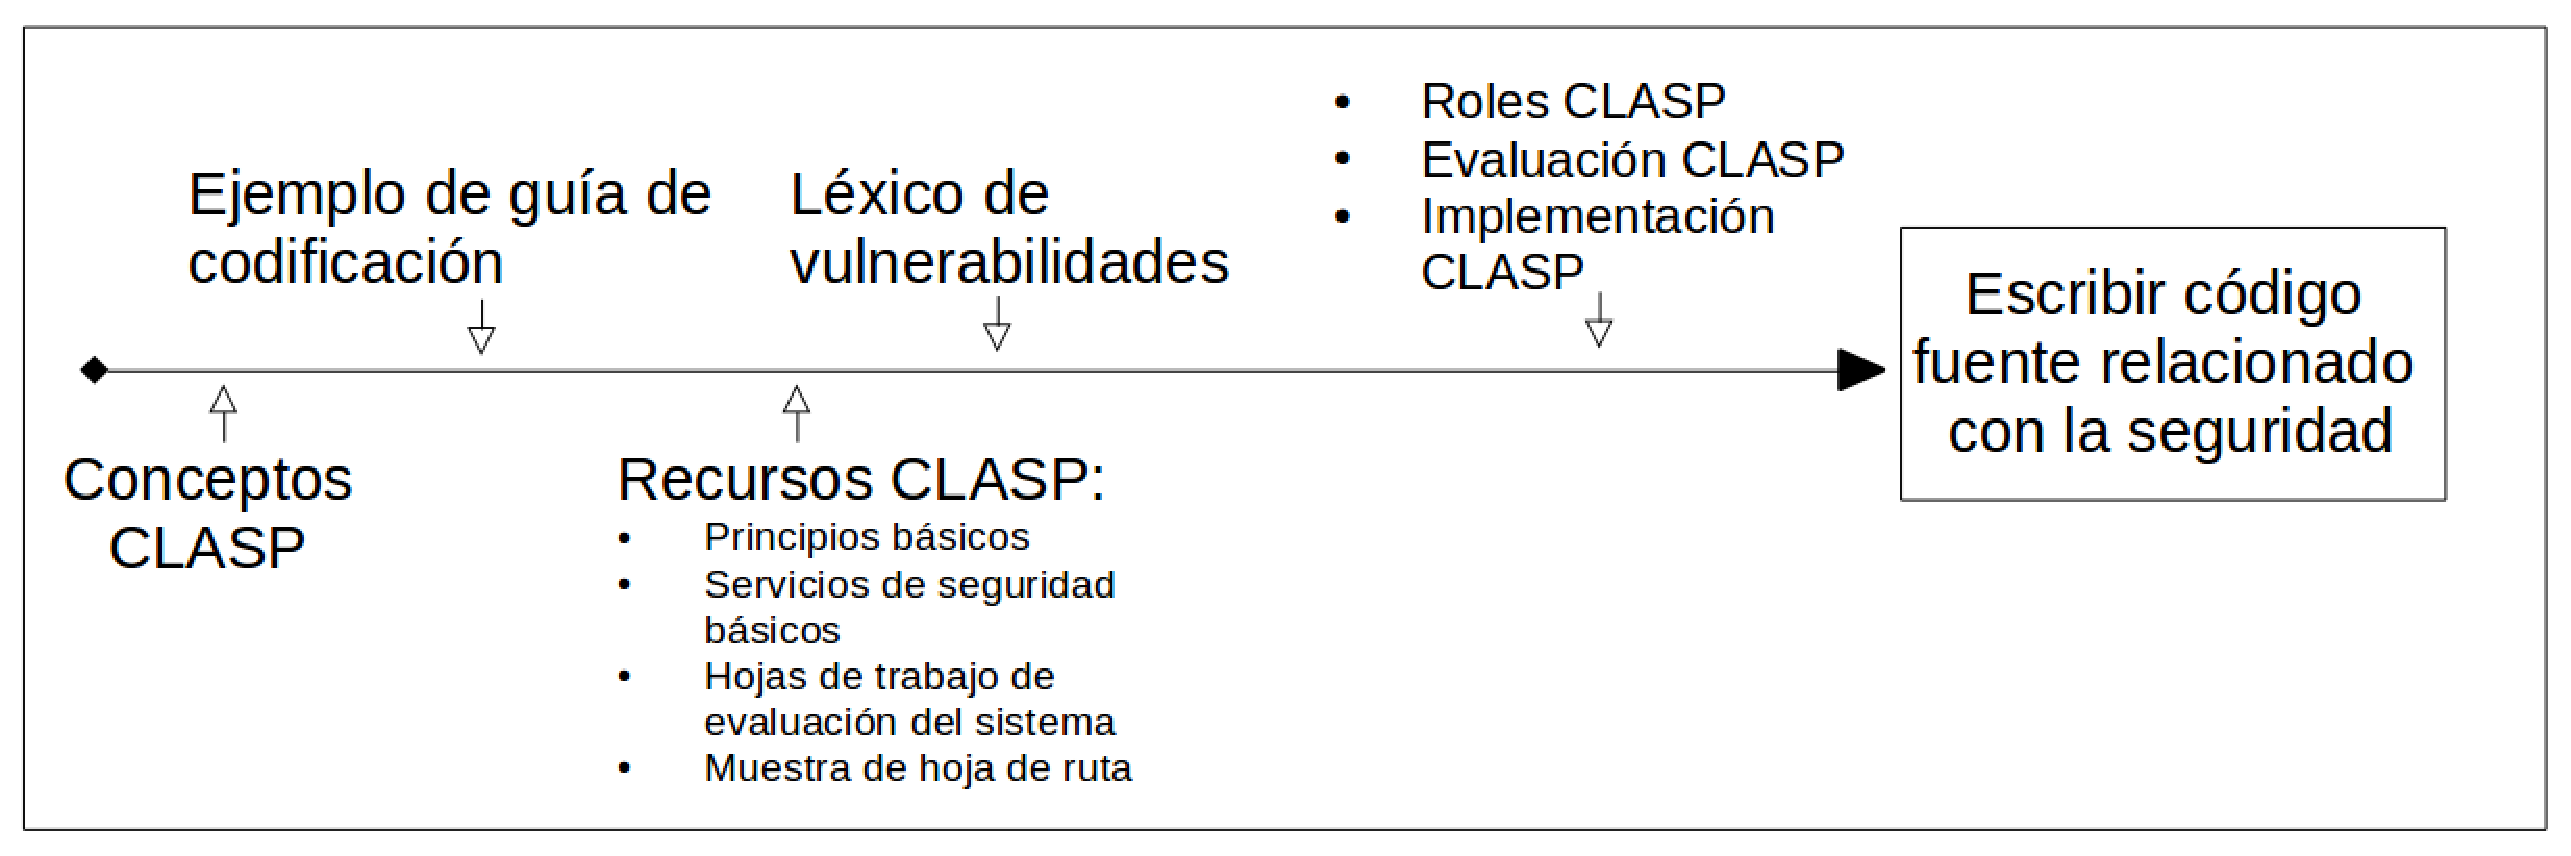
\includegraphics[height=6.0cm, width=12.0cm]{sa_figura_13}
\caption{Posible secuencia al aplicar los componentes \gls{CLASP} en un \gls{CVDS} definido.}
\label{fig:example}
\end{figure}

Una vez que se ha logrado el entendimiento de la \gls{VC} sera necesario continuar con el proceso de adopción  por medio de la comprensión de la siguiente información proveída por \gls{CLASP} \cite{CLASPIntroduction}.
\\
\begin{enumerate}
	\item Las 7 practicas que definen \gls{CLASP}.
	\item Resumen de los servicios de seguridad de alto nivel.
	\item Núcleo de principios de seguridad para el desarrollo de \gls{Software}.
	\item Roles que son incluidos en el desarrollo de \gls{Software}.
	\item Colección de actividades para construir \gls{Software} mas seguro.
	\item Asesoría del proceso de ingeniería \gls{CLASP} y mapas de ruta. 
	\item Lista de guías de codificación para ayudar a los desarrolladores y auditores con las revisiones de código.
	\item Léxico de vulnerabilidades.
	\item Glosario de términos y frases comunes para la aplicación de la seguridad.
	\item Lista de vulnerabilidades.\\
	
\end{enumerate}
Ademas del correcto entendimiento de la información proveída por \gls{CLASP} en la lista anterior sera necesario que los miembros del equipo conozcan a fondo el contenido de las 4 vistas restantes con el fin de generar una alto grado de eficacia a la hora de la total adopción de las piezas \gls{CLASP}. 

\subsubsection{¿Cómo evaluar \gls{CLASP}?}
\gls{CLASP} en su \gls{VBEA} provee la información necesaria para realizar evaluaciones sobre el desempeño de las actividades realizadas con el fin de mejorar la seguridad de los productos, en particular esta vista provee la siguiente información acerca de cada nueva actividad relacionada a las evaluaciones \cite{AAViewCLAPS}:

\begin{enumerate}
	\item Propósito de la actividad
	\item Responsable de la actividad
	\item Contribuidores
	\item Aplicabilidad
	\item Impacto relativo
	\item Riesgos por omisión
	\item Frecuencia de la actividad
	\item Horas hombre aproximadas para la actividad
	
\end{enumerate}
A continuación se presenta el formulario para el monitoreo de métricas propuesto en la \gls{VBEA} (véase figura 13).
\\

\begin{figure}
\centering
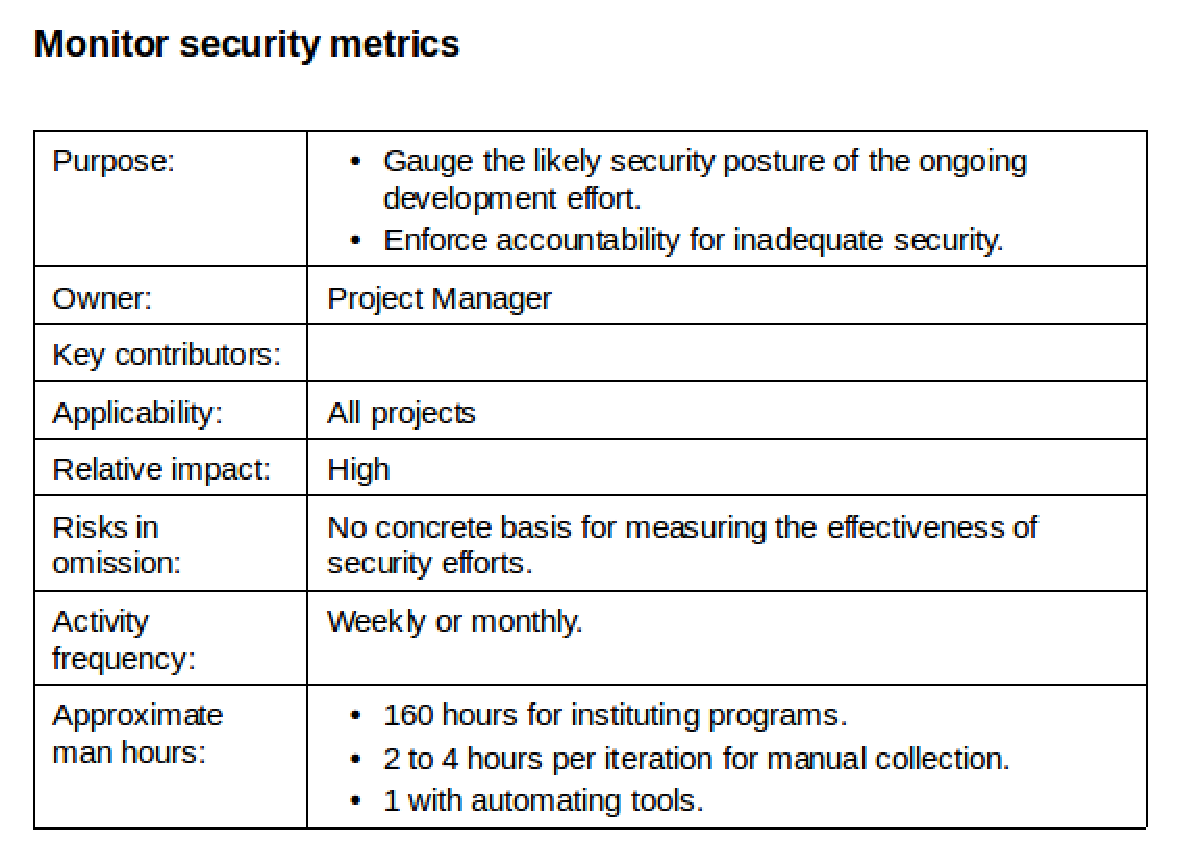
\includegraphics[height=10.0cm, width=12.0cm]{sa_figura_14}
\caption{Formulario para el monitoreo de métricas contenido propuesto en la \gls{VBEA}.}
\label{fig:example}
\end{figure}

Como soporte para al monitoreo de métricas \gls{OWASP} provee una sección en la cual es posible encontrar información relacionada con los siguientes aspectos.

\begin{enumerate}
	\item ¿Cómo identificar las métricas que deben de ser recolectadas?
	\item ¿Cómo identificar como serán usadas las métricas recolectadas?
	\item ¿Cómo recopilar datos?
	\item ¿Cómo realizar una estrategia para la presentación de informes?
	\item ¿Cómo recopilar y evaluar las métricas?\\
	
\end{enumerate} 
Por otra parte \gls{OWASP} propone el uso de \gls{SAMM} como modelo de madurez el cual es definido como un marco abierto para ayudar a las organizaciones a formular y poner en práctica una estrategia para la seguridad del \gls{Software} que se adapta a los riesgos específicos que enfrenta la organización \cite{SAMMIntroduction}.


\subsubsection{¿Quiénes deben poner en practica \gls{CLASP}?}
\gls{OWASP} provee una lista de entidades que en base a la experiencia obtenida a lo largo de varios años considera que deberían adoptar sus proyectos de seguridad entre ellos \gls{CLASP} \cite{OWASPIntroduction}.\\

A continuación son listadas dichas entidades.

\begin{enumerate}
	\item Desarrolladores de aplicaciones.
	\item Arquitectos de \gls{Software}.
	\item Autores e ingenieros de seguridad informática.
	\item Aquellos que quieran el apoyo de una comunidad profesional mundial para desarrollar o probar una idea.
	\item Cualquier persona que desee hacer uso de la organización profesional de los conocimientos \gls{OWASP}.
\end{enumerate}
\subsubsection{¿Cuáles son las cualidades de \gls{CLASP}?}
Las cualidades que \gls{CLASP} posee según el estudio realizado por Ikram El rhaffari y Ounsa Roudies y el cual esta enfocado en el análisis de elementos pertenecientes a la Ingeniería de \gls{Software}, a la Seguridad Informática y a las \gls{IT} y son listadas a continuación \cite{BenchmarkingSDLCLAPS}. 

\begin{enumerate}
	\item Cualidades relacionadas a la Ingeniería de \gls{Software}.
		\begin{enumerate}
			\item El producto final tendrá enfoque en la seguridad.
			\item La información para la implementación y los recursos necesarios se encuentran \gls{Online}.
			\item Es flexible.
			\item Posee su propia guía para el desarrollo de actividades.\\
			
		\end{enumerate}
	\item Cualidades relacionadas a la Seguridad Informática.
		\begin{enumerate}
			\item Posee un completo enfoque en la seguridad.
			\item Implica y compromete a un equipo de seguridad.
			\item Se implementa a través del \gls{CVDS}.
			\item Provee la información necesaria para el monitoreo y creación de métricas para la evaluación.\\
		\end{enumerate}
	\item Cualidades relacionadas con \gls{IT}.
		\begin{enumerate}
			\item Su documentación posee un alto indice de completitud y se encuentra disponible de manera \gls{Online}.
			\item Provee una completa cobertura organizacional.
			\item Se adapta fácilmente a pequeñas organizaciones.
		\end{enumerate}
\end{enumerate}

\subsubsection{¿Cuáles son las deficiencias que presenta \gls{CLASP}?}
Las deficiencias que \gls{CLASP} posee según el estudio realizado por Ikram El rhaffari y Ounsa Roudies y el cual esta enfocado en el análisis de elementos pertenecientes a la Ingeniería de \gls{Software}, a la Seguridad Informática y a las \gls{IT} y son listadas a continuación \cite{BenchmarkingSDLCLAPS}. 

\begin{enumerate}
	\item Deficiencias relacionadas a la Ingeniería de \gls{Software}.
		\begin{enumerate}
			\item El mapeo al \gls{CVTS} es complejo.
			\item No se alinea fácilmente con otros métodos de Ingeniería de Software.\\
			
		\end{enumerate}
	\item Deficiencias relacionadas a la Seguridad Informática.
		\begin{enumerate}
			\item Posee un bajo indice de cumplimiento y privacidad.\\
			
		\end{enumerate}
	\item Deficiencias relacionadas con \gls{IT}.
		\begin{enumerate}
			\item No se enfoca en la calidad de otros aspectos del producto.
			\item Evoluciona lentamente.
			\item No posee su propio modelo de madurez.
			\item Provee bajo soporte para el aseguramiento de la calidad de los servicios.\\
			
		\end{enumerate}
\end{enumerate}
\subsection{Metodo de Corrección por Construcción}
Correctness by Construction (CbyC, Corrección por Construcción), es un método radical que fusiona características de los \gls{Metodos Tradicionales} y los \gls{Metodos Agiles}. \gls{Praxis} ha puesto en practica \gls{CbyC} a lo largo de 12 años y a logrado obtener excelentes estadísticas de productividad, 0.05 defectos por cada 1,000 líneas de código y un aumento de alrededor de 30 líneas de código promedio por día por persona \cite{CbyCIntroduction}.   

\subsubsection{¿Qué es \gls{CbyC}?}
\gls{CbyC} es un método que se encuentra consolidado sobre 3 principios básicos que forman su eje principal, \gls{CbyC} posee características que permiten mejorar la calidad de la seguridad de los productos desarrollado y sus principios básicos son listados a continuación.

\begin{enumerate}
	\item Crear productos en los cuales sea muy difícil de introducir errores.
	\item Asegurar la eliminiación de los errores lo más pronto posible del punto de su introducción.
	\item Generar evidencia de aptitud para el propósito durante todo el desarrollo como un subproducto natural del proceso.
\end{enumerate}

En contraste con el método \gls{CbyD} que sigue siendo la forma en que la mayoría del \gls{Software} se desarrolla en la actualidad, \gls{CbyC} busca producir un producto correcto desde el inicio de su producción. La fase de pruebas se convierte en la demostración de sus características funcionales y no el punto de partida para la depuración pues se debe asegurar que los productos desarrollados integren las propiedades requeridas en lugar de sólo realizar pruebas y esperar por el defecto. \gls{CbyC} es un método técnico para el desarrollo de \gls{Software} altamente compatible con los principios de \gls{PSP} y \gls{TSP}. Evidencia tentativa de pequeña escala muestra que \gls{CbyC} combinado con \gls{PSP} y \gls{TSP} puede resultar en tasas de defectos aún más bajas. El enfoque técnico de \gls{CbyC} puede complementar \gls{PSP} para ofrecer altos indices de seguridad \cite{CbyCIntroduction}.\\ 

\gls{CbyC} posee 8 etapas o fases que poseen características propias de los \gls{Metodos Tradicionales} y los \gls{Metodos Agiles} (véase figura 14) \cite{CbyCBrito}. 

\begin{figure}
\centering
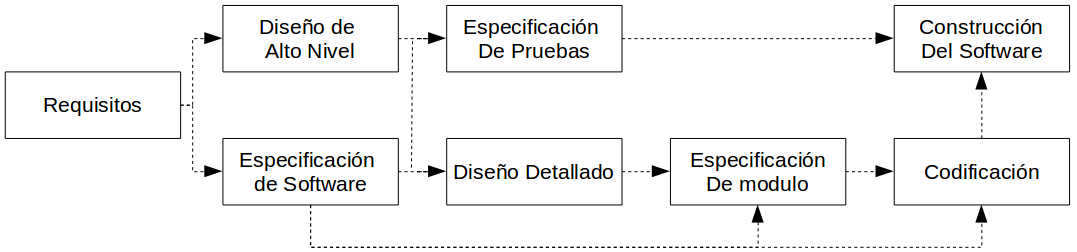
\includegraphics[height=4.0cm, width=12.0cm]{sa_figura_15}
\caption{Fases y secuencia de \gls{CbyC}.}
\label{fig:example}
\end{figure}

\begin{enumerate}
	\item Fase de Requisitos.\\
	
En esta fase se debe especificar el propósito del desarrollo, los requisitos no funcionales y 			  las funciones a desarrollar, se debe tomar en cuenta el diagramado por medio de técnicas y 				 	herramientas formales como \gls{Visual Paradigm} y \gls{UML} \cite{CbyCBrito}.\\
		  
		  \item Fase de Diseño de Alto Nivel.\\
		  
En esta fase es necesario describir la estructura interna del producto, se deben realizar 					  actividades tales como: distribuir de manera balanceada las funcionalidades a desarrollar, definir 			la estructura de las base de datos, definir los mecanismos para transacciones y comunicaciones así como priorizar los requisitos de protección y seguridad \cite{CbyCBrito}.\\
		  
		  \item Fase de Especificación del \gls{Software}.\\
		  
En esta fase se debe realizar la especificación de la interfaz del usuario, las especificaciones de los 		niveles superiores y desarrollar un prototipo para la validación \cite{CbyCBrito}.\\
		  
		  \item Fase de Diseño Detallado.\\
		  
En esta fase se debe definir los módulos, procesos y cada funcionalidad respectivamente, se deben tomar 		en cuenta el diagramado por medio de técnicas y herramientas formales como \gls{Visual Paradigm} y 			\gls{UML} \cite{CbyCBrito}.\\
		  
		  \item Fase de Especificación de Módulos.\\
		  
En esta fase se deben definir el estado y comportamiento de cada módulo teniendo un enfoque de bajo 			acoplamiento y alta cohesión \cite{CbyCBrito}.\\
		  
		  \item Fase de Codificación.\\
		  
En esta fase es necesario considerar el uso de un lenguaje que tenga características optimas para la comprobación matemática, en esta fase es necesario realizar pruebas estáticas y revisiones de código  \cite{CbyCBrito}.\\
		  
		  \item Fase de Especificación de Pruebas.\\
		  
En esta fase se debe considerar las Especificaciones de \gls{Software}, los Requisitos y el Diseño de Alto Nivel para realizar pruebas de comportamiento y pruebas que cubran los requisitos no funcionales. \cite{CbyCBrito}.\\
		  
		  \item Fase de Construcción del \gls{Software}.\\
		  
Considerando que \gls{CbyC} utiliza técnicas de \gls{Metodos Agiles}, la primera entrega debe 				contener un producto con todas las interfaces y mecanismos de comunicación, la funcionalidad del 			  producto se debe incrementar conforme a cada interacción \cite{CbyCBrito}.
		  
\end{enumerate}
\gls{CbyC} depende del conocimiento exacto sobre lo que el producto debe o no hacer y cuales características son prioritarias debido a esto se debe tener muy en claro que tipo de producto se esta desarrollando, si algún miembro del equipo de desarrollo lo desconoce esto podría ser causa de la inserción de defectos inesperados \cite{CbyCComercialSystem}.\\

CbyC incluye actividades de carácter genérico y entre las cuales se encuentran las siguientes.

\begin{enumerate}
	\item Planificación de procesos.
	\item Capacitación del personal.
	\item Trazabilidad de los requisitos a traves de la especificación de código y casos de prueba.
	\item Gestión de fallos.
	\item Gestión de cambios.
	\item Gestión de la configuración.
	\item Recolección de métricas.
\end{enumerate} 

\subsubsection{¿Porqué adoptar \gls{CbyC}?}
CbyC combina notaciones matemáticamente rigurosas con enfoques ágiles para el desarrollo gradual; el resultado es que la industria obtendrá bajas tasas de defectos combinados con una alta productividad.
La experiencia obtenida por \gls{Praxis} indica que la mejora de la calidad y la seguridad de los productos es notoria así como la productividad de cada uno de los miembros del equipo de desarrollo \cite{CbyCIntroduction}.

\subsubsection{¿Cómo adoptar \gls{CbyC}?}
Para lograr la correcta adopción de \gls{CbyC} es necesario que los miembros del equipo de desarrollo comprendan el flujo del proceso así como las características de cada etapa. Es importante mencionar que el dominio de \gls{Metodos Tradicionales} de desarrollo de \gls{Software} como \gls{PSP} y \gls{TSP} potenciaran la rápida adopción de \gls{CbyC} pues este posee características propias de dicho métodos. Ademas de ello los miembros del equipo de desarrollo deberán tener un solido conocimiento sobre los siguientes puntos. 

\begin{enumerate}
	\item Especificaciones precisas.\\
	
	Las especificaciones precisas y el dominio de lenguajes de programación comprobables matemáticamente como
	\gls{SPARK} son considerados obligatorios pues el cometido principal que se pretende obtener es eliminar
	cualquier ambigüedad, si se adopta \gls{CbyC} omitiendo los pre-requisitos para le desarrollo
	anteriormente mencionados solo quedaran las buenas practicas provistas por los \gls{Metodos Agiles},
	\gls{CbyC} captura esta idea con la frase "Write Right" \cite{CbyCIntroduction}.\\

	\item Validación robusta.\\
	
	Debido a que \gls{CbyC} utiliza notaciones no ambiguas es posible utilizar metodos para validar los
entregables de cada una de las etapas. Por ejemplo se puede demostrar que la especificación formal tiene
ciertas propiedades de seguridad necesarias, que el código fuente está libre de errores de tiempo de
ejecución, y que el código fuente implementa correctamente propiedades clave de la especificación
considerando hacer valido el principio de la detección temprana de errores. \gls{CbyC} captura esta idea
con la frase "Check Here Before Going There" \cite{CbyCIntroduction}.\\
	
	\item Desarrollo incremental.\\
	
	\gls{CbyC} considera den los productoos ideas que se complementan, la primera es acerca de la minimizacion de las
brechas semánticas entre artefactos por medio de la detección temprana de errores (ejemplo: sera difícil
predecir el comportamiento del código generado de un mal diseño),la segunda es acerca de el incremento
gradual de características considerando que el primer entregable sera el esqueleto gráfico completo del
producto así como los mecanismos de comunicación, la funcionalidad real deberá ser alcanzada gradualmente
de esta manera el sistema puede ser probado y demostrado desde el principio, que es una importante medida
de fomento de la confianza. Es posible combinar pequeñas brechas semánticas entre componentes,
anotaciones precisas y validaciones robustas y lograr generar pruebas de certificación como un subproducto.  \gls{CbyC} captura esta idea con la frase "Step, Don’t Leap" \cite{CbyCIntroduction}.\\

	\item Evitar la repetición.\\
	
	La repetición es la segunda causa de la inserción de defectos situada abajo de los diseños con ambigüedades, se debe considerar que si existen descripciones dobles o información repetida provocara confusión en el equipo de desarrollo pues es regular que los datos varíen en cada una, debido a esto es necesario evitar repetir documentos de diseño ademas se debera considerar hacer documentos detallados solo cuando sea inevitable. \gls{CbyC} captura esta idea con la frase "Say Something Once, Why Say It Again?" \cite{CbyCIntroduction}.\\ 

	\item Luchar por la simplicidad.\\
	
	Sera necesario que los miembros del equipo mantengan simple cada aporte realizado al proyecto. \gls{CbyC} captura esta idea con el acrónimo \gls{KISS} \cite{CbyCIntroduction}.\\ 
	
	\item Gestión de riesgo.\\
	
	Sera necesario desarrollar las partes menos obvias del sistema de esta manera se pretenden atacar los defectos con mayor nivel de complejidad cuando se tiene un mayor rango de recursos (tiempo y opciones de diseño) a disposición. \gls{CbyC} captura esta idea con la frase "Do The Hard Things First" \cite{CbyCIntroduction}.\\ 
	
	\item Pensar duro.\\
	
	\gls{CbyC} subraya que el razonamiento lógico debe demostrar la aptitud para lograr el propósito del sistema. Un sistema desarrollado de esta manera debe ser certificable a cualquier seguridad aplicable o estándar de seguridad. \gls{CbyC} captura esta idea con la frase "Argue Your Corner and Screws? Use A Screwdriver, Not A Hammer" \cite{CbyCIntroduction}.\\ 
	
\end{enumerate}


\subsubsection{¿Cómo evaluar \gls{CbyC}?}
Debido a la naturaleza del proceso y su amplia relación con métodos tradicionales como \gls{PSP} y \gls{TSP}  es posible utilizar las métricas que estos \gls{Metodos Tradicionales} proponen, entre ellas., la cantidad de defectos inyectados en cada fase, la cantidad de defectos mitigados en cada fase, entre otros. \gls{CbyC} propone como actividad genérica la recolección de métricas sin embargo no existe información de carácter publico que resuelva este problema.

\subsubsection{¿Quiénes deben poner en practica \gls{CbyC}?}
\gls{Praxis} se ha convertido en el principal promotor de \gls{CbyC} y propone como principales objetivos de mercado a organizaciones con los siguientes rubros \cite{CbyCPraxis}.

\begin{enumerate}
	\item Ferroviaria. 
	\item Aeroespacial.
	\item Milicia.
	\item Nuclear.
	\item Administración de trafico aéreo.
\end{enumerate}


\subsubsection{¿Cuáles son los beneficios que ofrece \gls{CbyC}?}
Los beneficios que aporta \gls{CbyC} según \gls{Praxis} se listan a continuación \cite{CbyCHighIntegritySystems}.

\begin{enumerate}
	\item Alta productividad pues el enfoque ahorra esfuerzo significativamente en el desarrollo de pruebas.
	\item \gls{Software} con pocos defectos pues los resultados refieren la existencia de muy pocos errores después de la entrega.
	\item \gls{Software} Garantizado pues la confianza se refleja en un estándar propio de garantía de software.
	\item Bajos costos de apoyo el \gls{Software} es fácil de mantener, con defectos fijos por garantía.
	\item Los clientes satisfechos el enfoque está orientado hacia el cumplimiento de los requisitos de negocio subyacentes del cliente.
\end{enumerate}

Las cualidades que \gls{CbyC} posee considerando los puntos propuestos por Ikram El rhaffari y Ounsa Roudies en su estudio y el cual esta enfocado en el análisis de elementos pertenecientes a la Ingeniería de \gls{Software}, a la Seguridad Informática y a las \gls{IT} y son listadas a continuación.  

\begin{enumerate}
	\item Cualidades relacionadas a la Ingeniería de \gls{Software}.
		\begin{enumerate}
			\item El producto final tendrá enfoque en la seguridad.
			\item Fácil trazabilidad a las fases de \gls{CVTS}.
			\item Se alinea con otros métodos de ingeniería de \gls{Software}.\\
			
		\end{enumerate}
	\item Cualidades relacionadas a la Seguridad Informática.
		\begin{enumerate}
			\item Posee un completo enfoque en la seguridad.
			\item Implica y compromete a un equipo de seguridad y su interacción con otros actores del desarrollo.
			\item Se implementa a través del \gls{CVDS}.
			\item Cumple con las necesidades de privacidad y confianza.\\

		\end{enumerate}
	\item Cualidades relacionadas con \gls{IT}.
		\begin{enumerate}
			\item Tiene un enfoqué en la calidad pues utiliza técnicas de \gls{PSP} y \gls{TSP}. 
			\item Provee una completa cobertura organizacional a través de las técnicas de \gls{PSP}, \gls{TSP} y \gls{CMMI}.
			\item Se adapta fácilmente a pequeñas organizaciones.
			\item Provee las características necesarias para evolucionar dentro de la organización.
			\item Es posible la combinación de lineamientos \gls{CMMI} para la evaluaciond e niveles de madurez.
			\item Provee amplia cobertura a diferentes estructuras organizaciónales.
		\end{enumerate}
\end{enumerate}
     
\subsubsection{¿Cuáles son las deficiencias que presenta \gls{CbyC}?}
Las deficiencias que \gls{CbyC} posee considerando los puntos propuestos por Ikram El rhaffari y Ounsa Roudies en su estudio y el cual esta enfocado en el análisis de elementos pertenecientes a la Ingeniería de \gls{Software}, a la Seguridad Informática y a las \gls{IT} y son listadas a continuación \cite{BenchmarkingSDLCLAPS}.

\begin{enumerate}
	\item Deficiencias relacionadas a la Ingeniería de \gls{Software}.
		\begin{enumerate}
			\item Pocos recursos informativos disponibles. 
			\item Es un proceso considerado riguroso.
			\item No existe una guía detallada para la realización de sus actividades.\\
			
		\end{enumerate}
	\item Deficiencias relacionadas a la Seguridad Informática.
		\begin{enumerate}
			\item Es posible realizar en análisis de métricas sin embargo solo es propuesto como actividad genérica y existe detalles sobre como llevarlo acabo.\\
			
		\end{enumerate}
	\item Deficiencias relacionadas con \gls{IT}.
		\begin{enumerate}
			\item Solo existen datos informativos y no descriptivos.
			\item Posee un un soporte deficiente para el aseguramiento de la calidad.
			
		\end{enumerate}
\end{enumerate}

\subsection{Proceso de Ingeniería de Requisitos de Seguridad}
Security Requirements Engineering Process (SREP, Proceso de Ingeniería de Requisitos de Seguridad), describe como deben de ser integrados los requisitos de seguridad en el proceso de ingenieria de \gls{Software} de manera sistemática e intuitiva. \gls{SREP} describe cómo integrar el \gls{CC} en el de ciclo de vida de desarrollo del \gls{Software} \cite{SREPMellado}.  

\subsubsection{¿Qué es \gls{SREP}?}
\gls{SREP} es un método para el establecimiento de requisitos de seguridad en el desarrollo de \gls{SIS} el cual esta basado en activos y es impulsado por riesgos. Describe cómo integrar el \gls{CC} en el de ciclo de vida de desarrollo del \gls{Software} por medio de la integración de un repositorio de recursos de seguridad que soporta el re-uso de requisitos, activos, amenazas y contra-medidas  \cite{SREPMellado}.\\

\gls{SREP} posee 9 actividades así como varias interacciones, cada interacción tendrá como resultado avances internos o externos de varios artefactos que funcionaran como la linea base de proceso \cite{SREPMellado}.

\begin{enumerate}
	\item Realizar acuerdo sobre definiciones.\\
	
	En esta actividad sera necesario establecer un criterio común de entendimiento sobre las definiciones de seguridad que serán empleadas, así como las políticas de seguridad organizacionales y la visión de la seguridad del \gls{SIS}. El documento de visión de la seguridad deberá ser escrito, en el se deberá hacer hincapié en la indicación del activo mas importante, la información \cite{SREPMellado}.\\
	
	\item Identificar activos críticos o vulnerables.\\
	
	En esta actividad se debe de considerar en primera instancia como activo mas valioso la información contenida en el sistema, ademas de ello se deberán valorar otros activos (dinero, productos tangibles o intangibles) según sea el caso y el enfoque del propio sistema \cite{SREPMellado}.\\
	
	\item Identificar objetivos de seguridad y sus dependencias.\\
	
	En esta actividad es posible utilizar el \gls{SRR}, si alguno de los activos identificados en la actividad anterior es parte del \gls{SRR} sera posible re-utilizar los objetivos de seguridad, de lo contrario sera necesario determinar los objetivos para cada nuevo activo así como los requisitos legales y las limitaciones presentadas en las leyes del país donde se desarrollara el sistema \cite{SREPMellado}.\\
	
	\item Identificar amenazas y desarrollar artefactos.\\
	
	Si los activos identificados en la actividad anterior forman parte del \gls{SRR} sera posible re-utilizar las amenazas asociadas, de lo contrario las nuevas amenazas podrían prevenir el objetivo de seguridad siendo logradas por medio de la instanciación de los casos de uso del negocio en casos de mal uso o instanciando los arboles de amenazas y ataques asociados con el negocio y el patrón de aplicación \cite{SREPMellado}. \\
	
	\item Evaluar de riegos.\\
	
	Una vez identificadas las amenazas se deberá determinar la probabilidad de correncia de cada amenaza así como evaluar su impacto y su riesgo de cada una, para llevar a cabo esta actividad es necesario utilizar la técnica propuesta por la \gls{MAGERIT} la cual se basa en tablas de análisis \cite{SREPMap}.\\
	
	\item Obtener requisitos de seguridad.\\
	
	En esta actividad cada objetivo de seguridad debe ser analizado para asegurar su relevancia en conjunto con una lista de amenazas que impliquen mayor riesgo, esto con el fin de seleccionar los requisitos de seguridad adecuados para la depuración de amenazas con respecto a la evaluación de riesgos. Después sera necesario transformar los objetivos de seguridad (Confidencialidad, Integridad, Disponibilidad, Autenticidad, Responsabilidad) en limitantes sobre las operaciones que se utilizan en los requisitos funcionales  \cite{SREPMellado}.\\
	
	\item Categorizar y priorizar los requisitos.\\
	
	De acuerdo con el impacto y la probabilidad de las amenazas y según el riesgo, se debe clasificar los requisitos de seguridad en categorías por medio de la creación de taxonomías.\\
	
	\item Inspección de requisitos.\\
	
	En esta actividad se deberá generar un reporte de validación. Por lo tanto sera necesario evaluar la calidad de los trabajos anteriormente realizados considerando los requisitos de aseguramiento de \gls{CC} y los cuales fueron establecidos en conjunto con todos los interesados en la primera actividad, después se deberá realizar la primera version del \gls{SRRD} con la ayuda de las clases de aseguramiento de \gls{CC} mostrando que todos los requisitos de seguridad se cumplen y que se logran todos los objetivos de seguridad, que el problema de seguridad definido anteriormente se resuelve, que todas las amenazas han sido
contrarrestadas, que las políticas de seguridad de la organización se hacen cumplir y que todos los supuestos
se cumplen \cite{SREPMellado}.\\
	
	\item Mejora del \gls{SRR}.\\
	
	En esta actividad se debera añadir al \gls{SRR} los nuevos elementos (amenazas genericas y especificas, requisitos desarrollados en la actividad 4 y 6), posteriormente se debera crear el \gls{STD} del \gls{CC} \cite{SREPMellado}.	
	
\end{enumerate}

\subsubsection{¿Porqué adoptar \gls{SREP}?}

\gls{SREP} tiene como meta principal facilitar la reutilización de recursos, el proposito del desarrollo  con el reuso de requisitos es identificar las descripciones de los sistemas que se podrían utilizar (total o parcialmente) con un número mínimo de modificaciones, reduciendo de este modo el esfuerzo total de desarrollo. La reutilización de requisitos de seguridad ayuda a aumentar la calidad: la inconsistencia, los errores, la ambigüedad y otros problemas pueden ser detectados y corregidos para una mejor utilización en proyectos posteriores. De esta manera, se garantiza la puesta en marcha de posibles ciclos de desarrollo rapidos basados en soluciones probadas \cite{SREPMellado2}.

\subsubsection{¿Cómo adoptar \gls{SREP}?}
\gls{SREP} describe detalladamente como integrar el \gls{CC} en el \gls{CVDS} en conjunto con el \gls{SRR} para promover el reuso de requisitos de seguridad que deberan ser modeloados por medio de las herramientas propuestas por \gls{UMLSec}, \gls{SREP} promueve la utilización de las etapas propuestas por \gls{UP}, debido a esto es necesario que los equipos de desarrollo conozcan el funcionamiento de las herramientas externas utilizadas por \gls{SREP} \cite{SREPMellado2}. 

\subsubsection{¿Cómo evaluar el impacto de \gls{SREP}?}
Para lograr la correcta evaluación del impacto generado debido a la adopcion de \gls{SREP} es necesario recurir a las actividades propuestas por el \gls{CC} en su seccion numero 3, en dicha seccion se definen los criterios de evaluación de \gls{PP} y \gls{ST}, ademas se presentan los niveles de evaluación que deben ser utililzados, dicho niveles estan basados en una escala predefinida de calificacion y son llamados \gls{EAL} los cuales definen una escala para medir el aseguramiento de los componentes \gls{TOE} \cite{CCIntroduction}.\\

\gls{CC} establece los roles que deben ser incluidos en las actividades de evaluacioón y los cuales pueden ser mencionados de la siguiente manera \cite{CCIntroduction}.

\begin{enumerate}
	\item \gls{PO}
	\item Desarolladores
	\item Evaluadores de seguridad de productos \gls{IT}
\end{enumerate}

La evaluación ha sido el medio tradicional para la obtención del aseguramiento y es la base del enfoque de \gls{CC}. Las técnicas de evaluación pueden incluir, pero no están limitados a \cite{CCIntroduction}:

\begin{enumerate}
	\item Análisis y comprobación de procesos y procedimientos
	\item Comprobación de la aplicación de los procesos y procedimientos definidos
	\item Análisis de la correspondencia entre el diseño de representaciones \gls{TOE}
	\item Análisis del diseño de representación \gls{TOE} contra los requisitos
	\item Verificación de pruebas
	\item Anáslis y guia de documentos
	\item Análisis de pruebas funcionales desarrolladas y los resultados obtenidos
	\item Pruebas funcionales independientes
	\item Análisis de vulnerabilidades incluyendo hipotesis por defecto 
	\item Pruebas de penetración 
\end{enumerate}

Debido a que \gls{CC} tiene como meta aplicar en minimo esfuerzo requerido para porveer el nivel necesario para el aseguramiento de la evaluación, el incremento del esfuerzo se constituye de la siguiente manera \cite{CCIntroduction}:

\begin{enumerate}
	\item Alcance, es decir, el esfuerzo es mayor debido a que una parte mayor del producto se incluye.
	\item Profundidad,  es decir, el esfuerzo es mayor, ya que se implementa en un nivel más fino de diseño y detalle de implementación.
	\item Rigor, el esfuerzo es mayor, ya que se aplica de manera más estructurada y formal.
\end{enumerate}

\subsubsection{¿Quiénes deben poner en practica \gls{SREP}?}
La organizacion internacional de \gls{CC} para la certificacion de productos menciona que las organizaciones candidatas a la inserción de actividades de \gls{CC} son aquellas enfocadas en desarrollar productos ligados a las siguientes categorias \cite{CCStat}.

\begin{enumerate}
	\item Sistemas y dispositivos para el control de acceso
	\item Sistemas y dispositivos biometricos
	\item Sistemas  y dispositivos de protección de fronteras
	\item Proteccion de datos
	\item Bases de datos
	\item Sistemas y dispositivos de detección
	\item \gls{IC}, targetas inteligentes, sistemas y dispositivos relacionados con targetas inteligentes
	\item Sistemas de administración de llaves
	\item Sistemas con funciones multiples
	\item Sistemas y dispositivos realacionados con las redes
	\item Sistemas operativos
	\item Sistemas y dispositivos relacionados a firmas digitales
	\item Computación confiable 
\end{enumerate}

\subsubsection{¿Cuáles son los beneficios que ofrece \gls{SREP}?}
Las cualidades que \gls{SREP} posee considerando los puntos propuestos por Ikram El rhaffari y Ounsa Roudies en su estudio y el cual esta enfocado en el análisis de elementos pertenecientes a la Ingeniería de \gls{Software}, a la Seguridad Informática y a las \gls{IT} y son listadas a continuación.  

\begin{enumerate}
	\item Cualidades relacionadas a la Ingeniería de \gls{Software}.
		\begin{enumerate}
			\item El producto final tendrá enfoque en la seguridad.
			\item Se alinea con otros métodos de ingeniería de \gls{Software}.
			\item Las actividades que lo componene se encuentran descritas en las guías formales propuestas por \gls{CC} y \gls{UP}.\\
			
		\end{enumerate}
	\item Cualidades relacionadas a la Seguridad Informática.
		\begin{enumerate}
			\item Posee un completo enfoque en la seguridad.
			\item Implica y compromete a un equipo de seguridad y su interacción con otros actores del desarrollo debido al enofque interactivo adoptado de \gls{UP}.
			\item Cumple con las necesidades de privacidad y confianza.
			\item Sus metricas de seguridad se encuentran definidas por \gls{CC}.\\

		\end{enumerate}
	\item Cualidades relacionadas con \gls{IT}.
		\begin{enumerate}
			\item Tiene un enfoqué en la calidad pues utiliza técnicas de \gls{CC} y \gls{UP}. 
			\item Provee evolucion y versionamiento constante bajo la supervision de \gls{ISO}.
			\item Es posible el uso de \gls{CCEAL} para la evaluacion de niveles de madurez.
		\end{enumerate}
\end{enumerate}

\subsubsection{¿Cuáles son las deficiencias que presenta \gls{SREP}?}
Las deficiencias que \gls{SREP} posee considerando los puntos propuestos por Ikram El rhaffari y Ounsa Roudies en su estudio y el cual esta enfocado en el análisis de elementos pertenecientes a la Ingeniería de \gls{Software}, a la Seguridad Informática y a las \gls{IT} y son listadas a continuación \cite{BenchmarkingSDLCLAPS}.

\begin{enumerate}
	\item Deficiencias relacionadas a la Ingeniería de \gls{Software}.
		\begin{enumerate}
			\item No utiliza las fases estandar de desarrollo de \gls{Software} o \gls{CVTS}. 
			\item Existen uy pocos recursos informativos disponibles.
			\item Es de caracter riguroso.\\
			
		\end{enumerate}
	\item Deficiencias relacionadas a la Seguridad Informática.
		\begin{enumerate}
			\item Debe exitir una conciencia preliminar sobre la seguridad en la organización.\\
			
		\end{enumerate}
	\item Deficiencias relacionadas con \gls{IT}.
		\begin{enumerate}
			\item La documenación disponible se encuentra bajo cargos economicos.
			\item No provee impacto ornanizacional general pues solo se enfoca en el proceso de desarrollo de \gls{Software}.
			\item Es necesario acceder a soporte externo para asegurar los niveles de calidad.
			\item Se enfoca en ornizaciones con ciertos grados de madurez y potencial economico.
			
		\end{enumerate}
\end{enumerate}


\subsection{Modelado Conceptual de Seguridad}
Conceptual Security Modeling  (CoSMo, Modelado Conceptual de Seguridad), propuesto por Christine Artelsmair, Wolfgang Essmayr, Peter Lang, Roland Wagner y Edgar Weippl, \gls{CoSMo} fue diseñado para reducir la brecha resultante del trato pobre de la seguridad durante la realización de los requisitos de seguridad de desarrollo de software, segun \cite{CoSMoIntroduction} la importancia de la seguridad es subvaluada y considerada como una especie de complemento que será aplicado al sistema después del desarrollo.

\subsubsection{¿Qué es \gls{CoSMo}?}
Es un técnica de modelado conceptual, segun \cite{CoSMoIntroduction} esta constituida por requisitos y mecanismos de seguridad, cada requisito puede ser alcanzado por medio de uno o mas mecanismos de seguridad, esto resulta en una matriz requisitos/mecanismos, dichos requisitos y mecanismos deberan ser formulados como una abstraccion de alto nivel.\\

A continuación se presentan los requisitos y mecanismos considerados por \cite{CoSMoIntroduction} como los mas importantes.

\begin{enumerate}
	\item Autenticidad, Autenticación e Identificacion.\\
	
	Segun \cite{CoSMoIntroduction} la Autenticación aborda el requisito de aseguramiento de Autenticidad, la Autenticación puede tomar varias formas.
	
	\begin{enumerate}
		\item Autenticación general de la identidad / autenticación
		\item Autenticación del contenido del mensaje  / autenticación
		\item Autenticacion del origen del mensaje / autenticación\\
	\end{enumerate}
	
En \cite{CoSMoIntroduction} se menciona que la Autenticación general de la identidad es comunmente consevida por medio de la insercion de un nombre de usuario (\gls{Identificador}) y una clave (\gls{Password}). La Autenticación del contenido del mensaje se refiere al proceso de verificacion de la información contenida en el mensaje que fue enviado. La Autenticación del origen del mensaje se refiere al proceso de verificación del emisor y el origen de un mensaje, esto es logrado por medio de el mecanismo de Autenticación del origen del mensaje incluyendo los conceptos de: firmas digitales, certificados digitales y confianza con terceros.\\

	\item Integridad, Discreción y Privacidad.\\
	
De acuerdo con \cite{CoSMoIntroduction} existen dos tipos de restricciones que corresponden directamente a la Integridad y a la Discresción. En general, las restriciones de Integridad son reglas que administran la actulizacion de la informacion y la validación de los datos. Las restriciones de Discreción son reglas que administran la clasificacion de los datos y su acceso. Los dos tipos de restricciones se subdividen en subtipos: restricciones semanticas y restriciones de Control de Acceso.\\

Segun \cite{CoSMoIntroduction} las restricciones de la Integridad semantica permiten definir y mantener el correcto estado de la información durante la operación. Las restricciones de la Integridad del Control de Acceso son declaraciones explicitas que pretenden notificar la Autorización para la modificación de ciertos datos con el fin de proteger las modificaciones maliciosas o accidentales. Las restriciones de la discrecion semantica especifican los niveles en los cuales los datos y su asociacion son clasificados. Las restricciones de la Discresion del Control de Acceso especifican cuales usuarios estan autorizados para accesar a ciertos datos.\\

	\item Atorización, Control de Acceso y Disponibilidad.\\

En \cite{CoSMoIntroduction} se mensiona que la Autorización es la especificación de un conjunto de reglas acerca de "¿Quien tiene?, ¿Cual tipo de acceso?, ¿A que información?". El Control de Acceso es logrado por medio de procesdimiento que controlan la Autorización  limitando el acceso a los datos solo a usuarios autorizados, el Control de Acceso usualmente requiere de la Autenticación como prerequisito. La Autorización y el Control de Acceso se vinculan con los requisitos de Discreción y Privavidad de los \gls{IS}.\\

El control de acceso puede tomar control por medio de las siguentes formas:\\

\begin{enumerate}
	\item Control de Acceso discrecional.
	\item Control de Acceso obligatorio.
	\item Control de Acceso basado en roles.\\
\end{enumerate}

En \cite{CoSMoIntroduction} se dice que la Disponibilidad es el requisito de servir a los actores autorizados  con la información adecuada cuando esta sea requerida. Para lograr el aseguramiento de la Disponibilidad es necesario proteger la información de los actores no autorizados. Para mantener la información disponible es necesario controlar el acceso a los datos.\\  
	
	\item Rendicion de Cuentas, Auditoria y No Repudio.\\

De acuerdo a \cite{CoSMoIntroduction} la Rendición de Cuentas captura el requisito realacionado a la responsabilidad que los individuos tinen sobre las actividades relavantes de reguridad y el cual puede ser alcanzado por medio del mecanismo de Auditoria. El No Repudio es un caso particular de Rendicion de Cuentas  y es un requisito que sera logrado por medio de metodos de \gls{Criptografia}. Al mecanismo encargado de llevar registro de todas las actividades relacionadas a la seguridad por un usuario es llamado Auditoria. La Auditoria esta formada por dos componentes: la recolección y organización de los datos asi como el analisis de los datos para descubrir vulnerabilidades.\\

	\item Anonimato y Originalidad.\\
	
En \cite{CoSMoIntroduction} se define como Anonimato a la carencia de identidad y se menciona que existen dos enfoques para proveer de Aninimato en la red:\\

	\begin{enumerate}
		\item Servicios anonimos: basados en un sistema de trasporte no anonimo (capa 1 a 4 en \gls{OSI}).
		\item Redes anonimas: implementando la anonimidad en las capas bajas de \gls{OSI} y construyendo diferentes servicios sobre ella con Anonimato hasta cierto punto (por ejemplo, anonimato real, pseudo-anonimato, auto-identificación opcional).\\
	\end{enumerate}

En este punto es necesario considerar a la infraestructura como un mecanismo mas, el cual jugara un papel muy importante para el desarrollo de nuevos sistemas seguros.\\

	\item Validez.\\
	
En \cite{CoSMoIntroduction} se menciona que los contratos y firmas digitales poseen validez legal y que debe de ser considerarda cada una de las vulnerabilidades existentes de los metodos implementados. Para lograr alcanzar una correcta Validez en los \gls{IS} sera necesario considerar la integración de nuevas herramientas dentro de la infraestructura.\\

	\item \gls{Criptografia} y Mecanismos Criptográficos.\\

Segun \cite{CoSMoIntroduction} los Mecanismos Criptograficos mas frecuentes son:\\

	\begin{enumerate}
		\item Algoritmos de cifrado que protegen la Confidencialidad de los datos.
		\item Firmas digitales que provee de iIntegridad y Autenticidad.
		\item Funciones para la revision de la Integridad (\gls{Hash Functions}) usadas tipicamente en conección con firmas digitales.\\
	\end{enumerate}

	\item Certificados Digitales y Terceros Confiables.\\
	
En \cite{CoSMoIntroduction} se menciona que los Certificados Digitales son usados para proveer Autenticidad a los involucradosen la comunicación, por ejemplo: la certificación de una llave publica provee la confianza de un individuo u organización. Una \gls{CA} actua como un Tercero Confiable que garantiza el enlace seguro entre los involucrados.

\end{enumerate}

\subsubsection{¿Porqué adoptar el \gls{CoSMo}?}
El cometido principal de \gls{CoSMo} es solucionar la falta de una técnica de modelado conceptual apropiado para la seguridad, \cite{CoSMoIntroduction} identifica la necesidad de integrar ciertas consideraciones de seguridad dentro del proceso de modelado de \gls{Software} y realiza una contribucion doble, \cite{CoSMoIntroduction} menciona en primer lugar que el modelado conceptual abarca los requisitos y mecanismos de seguridad de alto nivel y como es que las consideraciones de seguridad se pueden integrar en el proceso de modelado conceptual mejorando el proceso de manera radical, en segundo lugar menciona que los requisitos frecuentes de seguridad  que claramente indican cuales mecanismos son utilizados para lograr su propio cumplimiento deben ser sistemáticamente archivados, mejorando asi el consumo de recursos como tiempo de investigación y desarrollo. 

\subsubsection{¿Cómo adoptar el \gls{CoSMo}?}
En \cite{CoSMoIntroduction} se menciona que al adoptar el \gls{CoSMo} es necesario el uso de herramietas tales como \gls{UML} ya que permiten el modelado de requisitos de seguridad a nivel conceptual por medio de  diagramas de casos de uso, \cite{CoSMoIntroduction} menciona que UML es fácil, comprensible y ayuda a construir un entendimiento común de un nuevo sistema, debido a esto se debera poseer un conocimiento adecuado para la construcion de diagramas de calidad. Es importante tener en cuenta que sólo exigen requisitos de seguridad y que no existe mecanismo alguno que especifique cómo lograr dichos requisitos. Segun \cite{CoSMoIntroduction} los diagramas de casos de uso pueden ser enriquecidos a nivel conceptual por medio de los requisitos descritos con anterioridad en la sección ¿Qué es \gls{CoSMo}?.

\subsubsection{¿Cómo evaluar el impacto del \gls{CoSMo}?}
\gls{CoSMo} no posee un metodo definido para su evaluación, sin embargo es posible inferir la posibilidad de evaluar la completitud de requisitos de seguridad por medio de la caparativa entre los requisitos necesarios para el sistema y aquellos logrados.

\subsubsection{¿Quiénes deben poner en practica el \gls{CoSMo}?}
\cite{CoSMoIntroduction} menciona que las organizacines que deben utilizar el \gls{CoSMo} son aquellas enfocadas en desarrollar sistemas ligados a las siguientes categorias entre otros:\\

\begin{enumerate}
	\item Sistemas y dispositivos de control de acceso.
	\item Sistemas y dispositivos confiables.
	\item Sistemas y dispositivos biometricos.
	\item Sistemas y dispositivos de comercio electronico.
	\item Sistemas y dispositivos bancarios.
\end{enumerate}

\subsubsection{¿Cuáles son los beneficios que ofrece el \gls{CoSMo}?}

\subsubsection{¿Cuáles son las deficiencias que presenta el \gls{CoSMo}?}



\subsection{Lenguaje Unificado de Modelado Afín a la seguridad}

\subsubsection{¿Qué es el Lenguaje Unificado de Modelado Afín a la seguridad?}

\subsubsection{¿Porqué adoptar el Lenguaje Unificado de Modelado Afín a la seguridad?}

\subsubsection{¿Cómo adoptar el Lenguaje Unificado de Modelado Afín a la seguridad?}

\subsubsection{¿Cómo evaluar el impacto del Lenguaje Unificado de Modelado Afín a la seguridad?}

\subsubsection{¿Quiénes deben poner en practica el Lenguaje Unificado de Modelado Afín a la seguridad?}

\subsubsection{¿Cuáles son los beneficios que ofrece el Lenguaje Unificado de Modelado Afín a la seguridad?}

\subsubsection{¿Cuáles son las deficiencias que presenta el Lenguaje Unificado de Modelado Afín a la seguridad?}


\subsection{Casos de Uso Incorrecto}

\subsubsection{¿Qué son los Casos de Uso Incorrecto?}

\subsubsection{¿Porqué adoptar los Casos de Uso Incorrecto?}

\subsubsection{¿Cómo adoptar los Casos de Uso Incorrecto?}

\subsubsection{¿Cómo evaluar el impacto de los Casos de Uso Incorrecto?}

\subsubsection{¿Quiénes deben poner en practica los Casos de Uso Incorrecto?}

\subsubsection{¿Cuáles son los beneficios que ofrecen los Casos de Uso Incorrecto?}

\subsubsection{¿Cuáles son las deficiencias que presentan los Casos de Uso Incorrecto?}


\subsection{Metodología de Pruebas de Seguridad de Código Abierto}

\subsubsection{¿Qué es la Metodología de Pruebas de Seguridad de Código Abierto?}

\subsubsection{¿Porqué adoptar la Metodología de Pruebas de Seguridad de Código Abierto?}

\subsubsection{¿Cómo adoptar la Metodología de Pruebas de Seguridad de Código Abierto?}

\subsubsection{¿Cómo evaluar la Metodología de Pruebas de Seguridad de Código Abierto?}

\subsubsection{¿Quiénes deben poner en practica la Metodología de Pruebas de Seguridad de Código Abierto?}

\subsubsection{¿Cuáles son los beneficios que ofrece la Metodología de Pruebas de Seguridad de Código Abierto?}

\subsubsection{¿Cuáles son las deficiencias que presenta la Metodología de Pruebas de Seguridad de Código Abierto?}


\subsection{Construcción de la Seguridad por Modelos de Madurez}

\subsubsection{¿Qué es la Construcción de la Seguridad por Modelos de Madurez?}

\subsubsection{¿Porqué adoptar la Construcción de la Seguridad por Modelos de Madurez?}

\subsubsection{¿Cómo adoptar la Construcción de la Seguridad por Modelos de Madurez?}

\subsubsection{¿Cómo evaluar la Metodología de Pruebas de Seguridad de Código Abierto?}

\subsubsection{¿Quiénes deben poner en practica la Construcción de la Seguridad por Modelos de Madurez?}

\subsubsection{¿Cuáles son los beneficios que ofrece la Construcción de la Seguridad por Modelos de Madurez?}

\subsubsection{¿Cuáles son las deficiencias que presenta la Construcción de la Seguridad por Modelos de Madurez?}


\subsection{Sistema de Calidad de Requisitos de Ingeniería}

\subsubsection{¿Qué es el Sistema de Calidad de Requisitos de Ingeniería?}

\subsubsection{¿Porqué adoptar el Sistema de Calidad de Requisitos de Ingeniería?}

\subsubsection{¿Cómo adoptar el Sistema de Calidad de Requisitos de Ingeniería?}

\subsubsection{¿Cómo evaluar el Sistema de Calidad de Requisitos de Ingeniería?}

\subsubsection{¿Quiénes deben poner en practica el Sistema de Calidad de Requisitos de Ingeniería?}

\subsubsection{¿Cuáles son los beneficios que ofrece el Sistema de Calidad de Requisitos de Ingeniería?}

\subsubsection{¿Cuáles son las deficiencias que presenta el Sistema de Calidad de Requisitos de Ingeniería?}



\printnoidxglossaries     
         
\bibliographystyle{ieeetr}
\bibliography{bibliography}


\end{document}
